% mn2esample.tex
%
% v2.1 released 22nd May 2002 (G. Hutton)
%
% The mnsample.tex file has been amended to highlight the proper use of
% LaTeX2e code with the class file and using natbib cross-referencing.
% These changes do not reflect the original paper by A. V. Raveendran.
%
% Previous versions of this sample document were compatible with the LaTeX
% 2.09 style file mn.sty v1.2 released 5th September 1994 (M. Reed) v1.1
% released 18th July 1994 v1.0 released 28th January 1994

\documentclass[letterpaper,useAMS,usenatbib]{"mn2e"}
%\documentclass[letterpaper,useAMS]{"mn2e"}
%LINUX version of the path
%\documentclass[useAMS,usenatbib,letterpaper]{"/media/blank/Macintosh
%HD/Users/karenyng/Library/texmf/tex/latex/commonstuff/mn2e"}

% If your system does not have the AMS fonts version 2.0 installed, then
% remove the useAMS option.
%
% useAMS allows you to obtain upright Greek characters.  e.g. \umu, \upi
% etc.  See the section on "Upright Greek characters" in this guide for
% further information.
%
% If you are using AMS 2.0 fonts, bold math letters/symbols are available
% at a larger range of sizes for NFSS release 1 and 2 (using \boldmath or
% preferably \bmath).
%
% The usenatbib command allows the use of Patrick Daly's natbib.sty for
% cross-referencing.
%
% If you wish to typeset the paper in Times font (if you do not have the
% PostScript Type 1 Computer Modern fonts you will need to do this to get
% smoother fonts in a PDF file) then uncomment the next line 
%\usepackage{Times}

%%%%% AUTHORS - PLACE YOUR OWN MACROS HERE %%%%%
\usepackage{hyperref}
\usepackage{amssymb}
\usepackage{graphicx}
\usepackage{amsmath}
\usepackage[amssymb]{SIunits} 
\usepackage{booktabs}
\usepackage{hhline}
\usepackage{breqn}
\usepackage{standalone}
\usepackage{dcolumn}
	\newcolumntype{d}[1]{D{.}{.}{#1}}
\usepackage{tabularx}
\usepackage{booktabs}
\graphicspath{{graphics/}}
\newcommand{\mc}[1]{\multicolumn{1}{c}{#1}} % handy shortcut macro
%-----------------------------------------------------------------------

\defcitealias{D13}{D13}
\defcitealias{Jee13}{J13}
\defcitealias{M12}{M12}
\defcitealias{Sifon13}{Sif\'{o}n 2013}
\def\apjl{ApJL }
\def\aj{AJ }
\def\apj{ApJ }
\def\pasp{PASP }
\def\spie{SPIE }
\def\apjs{ApJS }
\def\araa{ARAA }
\def\aap{A\&A }
\def\nat{Nature }
\def\mnras{MNRAS }
\def\mnrasl{MNRASL }
\providecommand{\eprint}[1]{\href{http://arxiv.org/abs/#1}{#1}}
\providecommand{\adsurl}[1]{\href{#1}{ADS}}
\providecommand{\ISBN}[1]{\href{http://cosmologist.info/ISBN/#1}{ISBN: #1}} 


%-----------------------------------------------------------------------
\title[The dynamics and merging scenario of ACT-CL
J0102-4915, El Gordo]{The dynamics and merging scenario of the galaxy cluster 
ACT-CL J0102-4915, 
El Gordo}
\author[K. Y. Ng et al.]{K. Y. Ng$^{1}$, W. A. Dawson$^{2}$, D. Wittman$^{1}$, J.
Jee$^{1}$, J. Hughes$^{3}$, F. Menanteau$^{3}$, C. Sif\'{o}n$^{4}$\\
(temporary order)\\
$^{1}$Department of Physics, University of California Davis, One Shields
Avenue, Davis, CA 95616, USA\\ 
$^{2}$Lawrence Livermore National Laboratory, P.O. Box 808, Livermore, CA
94551-0808, USA \\
$^3$Department of Physics \& Astronomy,
Rutgers University, 136 Frelinghysen Rd., Piscataway, NJ 08854, USA\\
$^{4}$Leiden Observatory, Leiden University, PO Box 9513, NL-2300 RA
Leiden, Netherlands\\}

\begin{document}
%%---------to adjust for the weird bottom margin-----------
%\voffset=-.8in \hoffset=.15in
\date{arXiV 666} \pagerange{\pageref{firstpage}--\pageref{lastpage}}
\pubyear{1988} \maketitle \label{firstpage}
%-----------------------------------------------------------------------
\begin{abstract} 
Merging galaxy clusters with radio relics provide rare insights to the merger
dynamics as the relics are created by the violent merger process. 
We demonstrate one of the first uses of the
properties of the radio relic
to reduce the uncertainties of the dynamical variables 
and determine 3D configuration of a cluster merger, ACT-CL J0102-4915, El Gordo. 
From the double radio relic observation and X-ray wake morphology, 
it is believed that El Gordo is observed shortly after the first
core-passage of the subclusters.
At a redshift of 0.87, El Gordo (M$_{200c} = 
2.75\times10^{15} \pm^{7.4}_{1.5}$ M$_{\sun}$) is one of the most massive
clusters discovered in the early universe. The two subclusters of El
Gordo has a mass ratio of around 2:1. 
The X-ray and weak-lensing data of El Gordo show an offset of X kpc between
the intercluster gas and the dark matter (DM) at $\sim$4 $\sigma$ level.
All these features of El Gordo make it part of a valuable class of
dissociative mergers that can probe the self-interaction of dark matter.
We employ a Monte Carlo simulation to investigate the three-dimensional (3D)
configuration and dynamics of El Gordo and provide a summary of the probability
density functions of the inferred variables. By making use the polarization
fraction of the radio relic, we are able to constrain the estimate of the
angle between the sky and the merger axis to be $\alpha = 21\degree
\pm^9_{11}$.
The relative 3D merger speed of El Gordo was found to be $\sim 2400 ~\kilo\meter~
\second^{-1}$. We put our estimates of the time-since-collision into
context and showed that if the time-averaged shock velocities $\gg 1400~
\kilo\meter~\second^{-1}$ in the center of mass frame, the two subclusters
are more likely to be moving away from each other than moving towards each other. 
Finally, we compare our simulation results with other merging clusters and
show that El Gordo has very similar dynamical properties as the Bullet
Cluster.
\end{abstract}
%-----------------------------------------------------------------------
\begin{keywords}
gravitational lensing -- dark matter -- cosmology: observations -- X-rays:
galaxies: clusters -- galaxies: clusters: individual (ACT-CL J0102-4915) --
galaxies: high redshift 
\end{keywords}

%-----------------------------------------------------------------------
\section{Introduction} 
Mergers of dark-matter-dominated galaxy clusters probes properties
of the cluster components like no other systems. 
Clusters of galaxies are made up of 80\% of dark matter in mass content, 
with a smaller  portion of intercluster gas($\sim 15\%$ in mass content), and
sparsely spaced galaxies ($\sim 2\%$ in mass content) (REF). During a merger of
clusters, the subclusters are accelerated to high speeds of several
thousand \kilo \meter~\second$^{-1}$. The offsets of different components
of the subclusters dissociate show how various interactions of the different
components are at work. Observables such as offset between dark
matter and the other components may suggest dark matter self-interaction
(REF).  
\par
%(The following sentence does not actually fit in this paragraph and
%I have to put it somewhere else) difference of the galaxy colors in a merging cluster from relaxed cluster can also verify effects of environment on galaxy evolution.
%%\textbf{background of El Gordo}
%\textbf{What literature exists for El Gordo.}

%van Weeren 2011a suggests that the double radio relic can provide clue to
%collisional parameters ???
El Gordo possesses a range of special features that allows us to constrain
the merger dynamics in multiple ways.  Ever since the discovery of El Gordo
in the Atacama Camera Telescope (ACT) survey (REF), there is an ongoing effort for
collecting comprehensive data for El Gordo.
From the spectroscopy and Dressler-Schecter test for the member galaxies  in Sif\'{o}n et al. (2013), El Gordo is confirmed to be a binary merger 
without significant substructures. This picture is further supported by the
weak lensing analysis by Jee et al. (2013). The weak lensing analysis shows
a mass ratio of $\sim$2:1  between the two main subclusters, named according to their location as the northeast (NW) and southeast (SE) subclusters respectively. 
(See Figure \ref{fig:config}). El Gordo has interesting intracluster medium morphology as shown in the X-ray. In the northwest, it shows a wake feature, i.e.,
depression in the X-ray emissivity, while in the southeast, it shows
highest X-ray emissivity indicative of a cold gas core southeast of the
wake. The cold gas core may have passed from the northwest to the southwest
to have caused this morphology (Menanteau et al. 2011, hereafter M12). 
The extended mass distribution of El Gordo also makes it a good
gravitational lens. Zitrin et al. (2013) have found multiple strong
gravitationally lensed images around the center region of El Gordo. 
On the outer skirt of El Gordo, strong radio emission is detected in
the NW and the SE respectively. These radio emission has steep spectral
index gradient and are identified as radio relic associated with shockwaves
created from a merger \citep{Lindner13}. 
\begin{figure}
	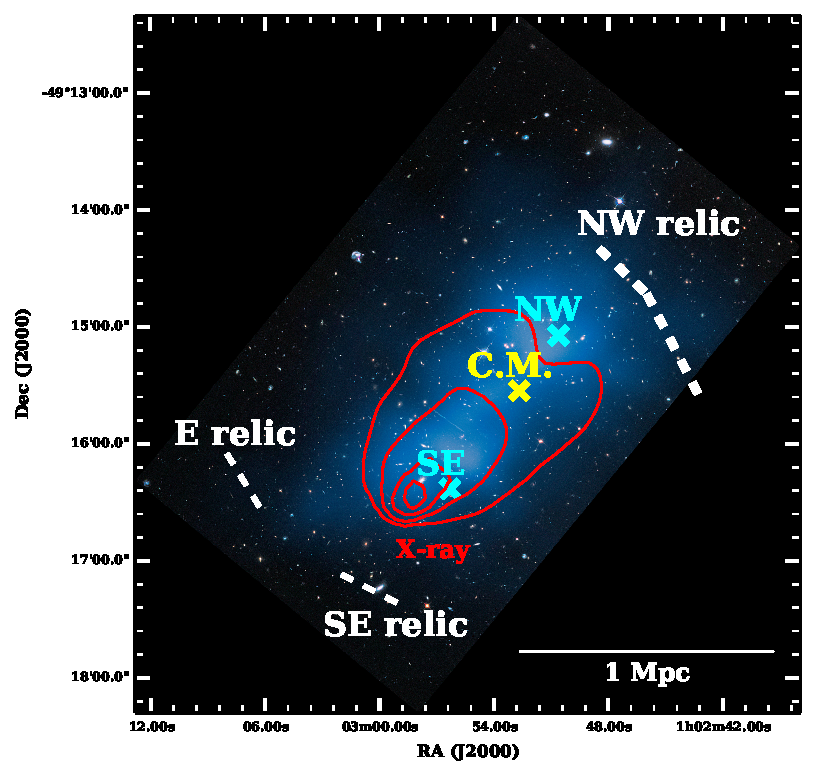
\includegraphics[width=\linewidth]{ElGordo.pdf}
	\caption{Configuration of El Gordo showing approximate overlaid of dark
		matter distribution in blue, and X-ray emissivity in red. The cross
		markers show the position of the northwest (NW) and southeast(SE) dark
		matter density peaks, and the center of mass (CM) location respectively.   
		The dashed white line indicates the approximate location of the northwest 
		radio relic (NW relic).
		(Image Credit: NASA, ESA and \citealt{Jee13} - not sure if I am citing
		the agencies in the appropriate format). 
		\label{fig:config}}
\end{figure}
El Gordo is one of small sample of galaxy clusters ($\sim 50$) that have
been associated with a radio relic and show dissociation between the X-ray
gas and the DM subclusters. Even fewer of them have been studied in
great details, making El Gordo a valuable candidate for further analysis.
\par 
In this paper, we combine available information of El Gordo with the main
goal of 1) inferring missing variables of the merger
such as the time-evolution and the 3D configuration, 2) giving estimates of
the associated dynamical parameters after taking into account all available
constraints and reflecting uncertainties due to the observed data.
Determining the time-since-collision of mergers of similar clusters helps
us reconstruct different stages of a cluster merger.
Mergers of clusters proceed on the time-scale of millions of year,
observations of each cluster only provides a snapshot of a particular type
of merger. In order to understand the merger process observationally, 
we need to identify different stages of similar dissociative mergers and
gather statistics to understand the physics of the mergers.  
Another crucial piece of missing information is the 3D
configuration, i.e. the angle between the plane of the sky and the merger
axis called the projection angle $\alpha$. Since most of the dynamical
observables are projected quantities while our physics require 3D
variables, the deprojection based on $\alpha$ contributes the
largest amount of uncertainties to the dynamical variables \citepalias{D13}.
From the morphology of the double relic of El Gordo, it is believed that
$\alpha$ should be small. For  mergers with a
large projection angle, the radio emission would be projected towards the
center of the merger, which is hard to be detected \citep{Vazza11}.
However, there has not been any quantitative constraints on the upper bound of $\alpha$.  
\par 
We employ a data-driven approach that thoroughly probes parameter
space by directly drawing samples from the observables. 
This work based on Monte Carlo simulation is particularly important since
it is forbiddingly expensive to simulate and analyze clusters similar to El
Gordo in high resolution. Previous attempts at modeling El Gordo with hydrodynamical
simulations such as \cite{Donnert13} and \cite{Molnar14} provided only in
total a dozen possible configurations of El Gordo, which could hardly be
representative of the input uncertainties. Their sophisticated but
specialized setup are more suitable for understanding the gas dynamics
rather than for estimating overall parameters. Another approach for
estimating dynamical parameters
would be to look for multiple analogs of El Gordo in cosmological
simulations.  However, under the hierarchical picture
of structure formation in the $\Lambda$CDM model, there is a rare chance
for massive clusters like El Gordo to have formed at a redshift of $z = 0.87$.  
The number density of analogs with mass comparable to El Gordo in a
cosmological simulation is as low as $10^{-11} \mega\text{pc}^{-3}$ \citepalias{M12}.  
\par

%Furthermore, El Gordo satisfies the four criteria for being a dissociative
%merger, which are proposed to be special probes of self-interacting dark matter (Dawson et al. 2012) . (1) The subclusters
%of El Gordo has a small ratio of mass, i.e. $\sim 2:1$ (Jee et al. 2013,
%hereafter J13). (2) The merger axis, the line joining the two subclusters,
%coincides with the alignment of the double radio relic propagating outward at the periphery of the cluster (Menauteau et al. 2012,
%hereafter M12). This suggests a simple merger configuration with small
%impact parameter.  (3) The X-ray luminosity peak is shown to be offset
%from the weak-lensing peak by X kpc at X $\sigma$ level (J13). (4) The
%observation of the double radio relic suggests that the angle between the
%merger axis and the plane of the sky has to be reasonably small (M12,
%Lindner et al. 2013), or else the relic may appear as a halo instead
%\citep{S13}. Each of these listed properties give us some basis to make
%simplifying assumptions for modeling El Gordo, and more importantly, to
%reduce the inferred parameter space of the dynamical variables. 
%\par 


%\textbf{motivation2}

In the following sections, we adopt the following conventions: (1) we
assume the standard $\Lambda$CDM cosmology with $\Omega_{m} = 0.3$, $\Omega_{\Lambda} = 0.7$. (2) All confidence intervals are quoted at the 68\% level unless otherwise stated. 
(3) All credible intervals (a.k.a. Bayesian confidence intervals that also
takes into account prior probability) are also
quoted at the 68\% level unless otherwise stated and are central credible
intervals. (4) All quoted masses ($M_{200c}$) are based on mass contained
within $r_{200}$ where the mass density is 200 times the critical density
of the universe ($\rho_{crit}$) at the redshift of $z = 0.87$. 
%-----------------------------------------------------------------------

\section{DATA} 
We gathered and analyzed data from multiple sources for different
purposes. For assigning membership of galaxies to the two identified subclusters, we
examined the spectroscopic data obtained from the Very Large Telescope (VLT) and
Germini South as described in \citetalias{M12} and \citet{Sifon13}.
For the weak-lensing mass estimation, we used the published
Monte Carlo Markov Chains (MCMC) mass estimates from \citetalias{Jee13}.
See Table~\ref{tab:inputs} for descriptions of the probability density
functions (PDFs) of the input
variables. \par 
%and these galaxies were discussed as the population in Region A in
%\citetalias{Jee13}.  
In order to further constrain our parameter space, we referred to the properties of
the radio relic from \citet{L13}. El Gordo shows radio relics on the
periphery of both subclusters \citepalias{M12}. Two radio relics, the
northwest (NW) relic and the southeast (SE) relic, of El Gordo were first
discovered in the Sydney University Molonglo Sky Survey (SUMSS) data in low
resolution at 843 MHz \citep{Mauch03} as shown in M12. The higher
resolution radio observation conducted by \cite{L13} at 610 \mega Hz and
2.1 \giga Hz confirms that the identity of the NW radio relic
after removing effects of radio point sources.The NW radio relic, which
possesses the most extended geometry (0.56 Mpc in length)
among all radio source, was identified to be associated with the
merger. We do not refer to the SUMSS SE nor the E radio relic in this paper
since the upstream velocity of those radio relics are not reported in
\citet{L13}.    
%\input{2.0_data_section.tex}

\section{METHOD -- Monte Carlo simulation} 
%For this analysis, we made use of the collisionless 
dark-matter-only Monte Carlo modeling code written by Dawson (2013),
hereafter \citepalias{D13}.  
In the code, the time evolution of the head-on merger was computed
analytically, assuming that the only dominant force is the gravitational attraction from
the masses of two truncated Naverro-Frenk-White (hereafter NFW) DM halos.
Other major assumptions for modeling systems with this code include
negligible impact parameter and no self-interaction of dark matter.\par

In the Monte Carlo simulation, many realizations of the collision is
computed from the inputs of each realization, including
the data ($\vec{D}$) and the model variable ($\alpha$). In particular,
the standard required data, which were in the form of samples of the probability density
functions (PDFs), included the masses ($M_{200_{NW}},M_{200_{SE}}$) the
redshifts ($z_{NW}, z_{SE}$) and the projected separation of the two
subclusters ($d_{proj}$).  
%For the $j-$th realization, w
In each realization, we randomly drew the samples of the PDFs.
%
%\begin{equation}
%	D_i^{j} \sim \mathcal{L}(\vec{\theta}|D_i) =  P(D_i | \vec{\theta})
%\end{equation}
%and we also draw the model variable $\alpha$ from the prior:
%\begin{equation}
%	\alpha^j \sim P(\alpha)
%\end{equation}
These inputs are then used for computing the output variables
($\vec{\theta}^\prime$) by making use of conservation of energy to describe
their collision due to the mutual gravitational attraction.
%\begin{equation}
%(\vec{\theta}^\prime)^{(j)} = f(\vec{D_i}^j, \alpha^j) 
%\end{equation}
%where $f$ are some suitable functions expressing the conservation of energy.
(See Table \ref{tab:inputs}
for quantitative descriptions of the sample PDFs and we outline how those
PDFs are obtained in the following subsections.) 
To ensure convergence of the output PDFs, in total, 2 million (to be
confirmed) realizations were computed. The results, however, are
consistent up to a fraction of a percent just from 20 000 runs
\citepalias{D13}.\par    
We note that the Monte Carlo simulation is written under a Bayesian
framework but differs from conventional Bayesian inference. The Bayes
chain rule underlies the simulation is:
\begin{equation}
    P(\vec{\theta}|\vec{D}) \propto P(\vec{D}|\vec{\theta})P(\vec{\theta})
\end{equation}
where the likelihood is defined to be the PDF of $\vec{D}$ given $\vec{\theta}$,
i.e. the input variables, not statistical parameters, and the priors are
defined to be the probabilities due to prior knowledge of the estimated values of
$\vec{\theta}$. The output variables $\vec{\theta}^\prime$, on the other
hand, were computed according to the conservation of energy, which is represented by a suitable
function form $f$ below. For example,the calculation of the $j$-th realization: 
\begin{equation}
    (\vec{\theta}^\prime)^{(j)} = f(\vec{\theta}^{(j)}, \vec{D}) 
\end{equation}    
The estimated values of $(\vec{\theta}^\prime)^{(j)}$ were then computed
over all $j$ realizations. Finally, we took physical
constraints on $\vec{\theta}$ and $\vec{\theta}^\prime$ into account by
excluding the unphysical realizations, and we refer to this process as
``applying prior probability''. 

%To model projection effects, we randomly draw a projection
%angle in each realization. We throw out realizations with unphysical
%outputs.  \textbf{what are the inputs}

We used the collisionless 
dark-matter-only Monte Carlo modeling code written by Dawson (2013),
hereafter \citepalias{D13}, to compute the physics of between
the first and second core-passage of the DM subclusters. 
In the D13 code, the time evolution of the
head-on merger was computed based on an analytical, dissipationless model
assuming that the only dominant force is the gravitational attraction from
the masses of two truncated Naverro-Frenk-White (hereafter NFW) DM halos. 
In the simulation, many realizations of the collision is
computed by drawing random realizations of the probability density
functions (PDFs) of the inputs, including
the data ($\vec{D}$) and one model variable, the projection angle between
the plane of the sky and the merger axis, $\alpha$. In particular,
the required data, included the masses ($M_{200_{NW}},M_{200_{SE}}$) the
redshifts ($z_{NW}, z_{SE}$) and the projected separation of the two
subclusters ($d_{proj}$).  
(See Table~\ref{tab:inputs}
for quantitative descriptions of the sample PDFs) 
Each set of inputs is then used for computing the output variables
($\vec{\theta}^\prime$) by making use of conservation of energy to describe
their collision due to the mutual gravitational attraction.
To ensure convergence of the output PDFs, in total, 2 million realizations
were computed. 
The results, however, are consistent up to a fraction of a percent just
from 20 000 runs \citepalias{D13}. The random sampling allows us to
throughly explore the multidimensional input parameter space and account
for the uncertainties of the inputs at the same time.
\par    


% NOT SURE IF IT IS A GOOD IDEA TO TALK ABOUT THIS
We adapt a Bayesian interpretation of the PDFs of the Monte Carlo
simulation. The Bayes chain rule underlies the simulation can be written as:
\begin{equation}
    P(M|\vec{D}) \propto P(\vec{D}|M)P(M)
\end{equation}
where the likelihood is defined to be the PDF of $\vec{D}$ given our
physical model $M$ which we parametrize using variables in Table 1
($\vec{\theta}$).
For example,the
calculation of the output variables of the $j$-th realization can be denoted as: 
\begin{equation}
    (\vec{\theta}^\prime)^{(j)} = f(\vec{\theta}^{(j)}, \vec{D}) 
\end{equation}    
and computed over all $j$ realizations. Finally, we took the physical
constraints on the dynamical variables into account by
examining the resulting physical variables against the physical limits and
excluding realizations that would produce impossible values. We refer to this
process of excluding unphysical realizations as applying priors. 
Even though we denote the priors for one dimension at a time (See Appendix~\ref{app:priors}), 
the correlations between different variables are properly taken into account
 due to how we throw away all the variables of problematic
realizations. 

The system of El Gordo satisfies several major assumptions in the Monte Carlo
simulation.
One of the strongest assumption is that all realizations correspond to
gravitationally bound systems. The simulation excludes all realizations
that would result in relative collisional velocities of the subclusters
higher than the free-fall velocity. The relative escape velocity of the
subclusters for El Gordo is $4500~\kilo\meter~\second^{-1}$ given
the mass estimates of \cite{Jee13} .  
Studies from cosmological simulations giving the PDFs of the pairwise velocities of massive merging clusters ($>
10^{15} M_{\sun}$) indicate that it is highly unlikely that the pairwise
velocities would $> 3000~\kilo \meter~\second^{-1}$ under $\Lambda$CDM.
(\citealt{Thompson12}, \citealt{Lee2010}).  Other major assumptions for
modeling systems with this code include negligible impact parameter. Even
though there are studies indicating that the impact parameter of El Gordo
may be as large as $300$ kpc $ \approx 40\% r_s$\citep{Molnar14},
where $r_s$ is the characteristic core
radius of the NFW halo with the mass of El Gordo. According to
\cite{Ricker98}, the resulting remnant of bimodal cluster mergers would only be
different when the impact parameter $> 10~ r_{\text{core}}$.
\cite{Maststropietro2008a} also reported that an impact parameter of $0.1
r_{200}$ affected merger dynamics only at the $\sim$10\% level.   
Other assumptions in this simulation include negligible dynamical friction
during the merger, negligible mass accretion and negligible self-interaction
of dark matter. Discussion of the effects of each of these assumptions are
included in \citetalias{D13}.  
\par

\subsection{Inputs of the Monte Carlo simulation} \label{sec: inputs}
\setcounter{table}{0} 
\setcounter{table}{0}
\begin{table}
\caption{Properties of the sampling PDFs of the Monte Carlo simulation} 
\begin{center} 
\begin{tabular}{@{}lcccc}
\hline \hline Data & Units & Location & Scale & Ref\\ \hline
$M_{200c_{\mathrm{NW}}}$ & $10^{14} h_{70}^{-1}$ M$_{\odot}$ &13.0&1.6& \citetalias{Jee13}\\ 
c$_{\mathrm{NW}}$ &  & 2.50& 0.02& \citetalias{{Jee13}} \\ 
$M_{200c_{\mathrm{SE}}}$ & $10^{14} h_{70}^{-1}$ M$_{\odot}$ &7.6&1.2 & \citetalias{Jee13}\\ 
$c_{\mathrm{SE}}$ &  & 2.70 & 0.04& \citetalias{Jee13}\\ 
$z_{\mathrm{NW}}$ &  & 0.86842 & 0.00109& \citetalias{M12}, \citetalias{Sifon13}\\ 
$z_{\mathrm{SE}}$ &  & 0.87110 & 0.00117& \citetalias{M12}, \citetalias{Sifon13}\\ 
d$_{\mathrm{proj}}$ & Mpc & 0.74 &0.007 & \citetalias{Jee13} \\ 
\hline 
\end{tabular} 
\end{center} 
\label{tab:inputs} 
\end{table} 



%-----------------------------------------------------------------------
\subsubsection{Membership selection and redshift estimation of subclusters}
%% \textbf{how do we determine the overall membership}
% relevant info of the membership is in M11 table 1
% cannot determine the membership of two galaxies 
% spatial cut is defined in M11 p.9 first paragraph 

% paragraphs needs to be reorganized 
We adopt the identification of galaxy membership of El Gordo given by
\citepalias{M11} with a total count of 89 galaxies.
%The overall membership of the galaxies
%of El Gordo was first determined using a shifting gapper method
%\citep{Fadda96} after applying a rest frame cut of
%4000~\kilo\meter~\second$^{-1}$ \citep{Sifon13}. This method gives a
To further distinguish member galaxies of each subcluster, we adopt a
redshift cut of $z < 0.886$, and a spatial cut approximately perpendicular
to the 2D merger axis from \citetalias{M11} to determine that
there are 51 members in the NW subclusters and 35 members in the SE subclusters (See Figure
\ref{fig:membership}). 
The spatial cut indicated by the green line was done after
mapping the world coordinates to pixel coordinates to avoid anamorphic distortion. 

%Compare and contrast the amount of bootstrapping and the reported
%redshifts and velocity dispersion.
After identifying members of each subcluster, we performed 10, 000 bootstrap realizations to estimate the biweight
locations of the redshifts of the respective members in order to obtain the
samples of the PDFs of the redshifts of each subcluster. 
The spectroscopic redshift of the subclusters were
determined to be 
%$z_{total} = \pm $ 
$z_{\mathrm{NW}} = 0.86842 \pm 0.0011$ and 
$z_{\mathrm{SE}} = 0.87131 \pm 0.0012$, where the quoted numbers represent the
biweight location and 1$\sigma$ biased corrected confidence level
respectively \citep{Beers90}.  
%These biweight location estimators are less susceptible to outliers than
%the mean and standard deviations. 
Both the estimated redshifts of the subclusters and the uncertainties are
consistent with estimates given by \citealt{Sifon13}, and the fact that El
Gordo shows large velocity dispersion and has the largest velocity
dispersion among all the ACT galaxy clusters as reported by
\citetalias{M13}. These redshifts of the subclusters correspond to a
radial velocity difference in the frame of the NW subcluster
to be $476 \pm 242 $ km/s. We estimate the radial velocity differences of the
subclusters by first calculating the velocity of each subcluster with
respective to us, using  
\begin{equation}
	v_i = \left[ \frac{(1+z_i)^2 - 1 }{(1+z_i)^2 + 1 }\right]c
\end{equation}
where $c$ is the speed of light. And then the radial velocity was calculated
by: 
\begin{equation}
	\Delta v_{rad}(t_{obs}) = \frac{|v_2 - v_1|}{1-\frac{v_1 v_2}{c^2}}
\end{equation}
This result is lower than the the quoted radial velocity differences of
$586$
km/s reported by \citetalias{M11} from the approximation of $\Delta v_{rad}
= c(z_1 - z_2) / (1 + z_1)$ in the frame of the NW subcluster. 


\begin{figure}
	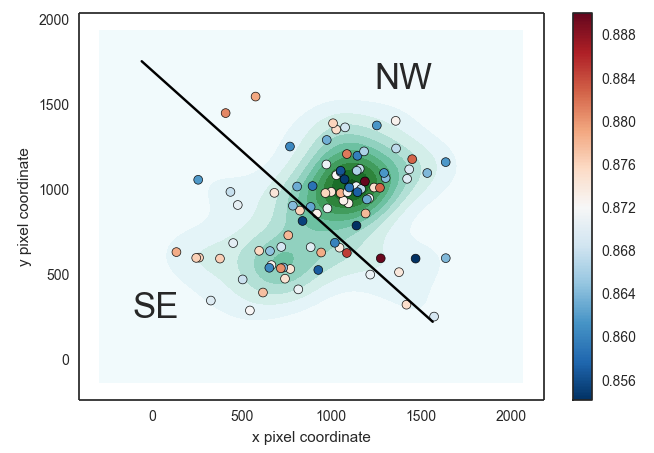
\includegraphics[width = \linewidth]{confirmed_member_divide.png}
	\caption{\label{fig:membership} The division of
the member galaxies among the two subclusters of El Gordo by a spatial cut
(green line). The color bar shows the color mapping of the spectroscopic
redshift of the member galaxies, with the redder end indicating higher
redshift.} 
\end{figure}

%We confirm the existence of the subclusters of El Gordo from the 2D spatial
%location of the galaxies, with the more massive cluster lying in the
%northwest (NW) and the less massive subcluster lying in the southeast(SE)  (REF - also have to reference the other literature
%for confirmation in the other wavelengths)
%
%Specifically, the membership of the NW and SE subclusters are
%determined based on a combination of the redshift and the spatial location. 

We adopt the identification of galaxy membership of El Gordo given by
\citetalias{M12} with a total count of 89 galaxies.
%The overall membership of the galaxies
%of El Gordo was first determined using a shifting gapper method
%\citep{Fadda96} after applying a rest frame cut of
%4000~\kilo\meter~\second$^{-1}$ \citep{Sifon13}. This method gives a
To further distinguish member galaxies of each subcluster, we adopt a
redshift cut of $z < 0.886$, and a spatial cut along (01:03:22.0,
-49:12:32.9) and (01:02:35.1, -49:18:09.8). The spatial cut is approximately perpendicular
to the 2D merger axis and are consistent with the bimodal number density
contours (See Figure~\ref{fig:membership}). We determined that
there are 51 members in the NW subclusters and 35 members in the SE
subclusters. 
The spatial cut indicated by the black line was done after
mapping the world coordinates to pixel coordinates to avoid anamorphic
distortion.  

%Compare and contrast the amount of bootstrapping and the reported
%redshifts and velocity dispersion.
After identifying members of each subcluster, we performed 10, 000 bootstrap realizations to estimate the biweight
locations of the spectroscopic redshifts of the respective members in order
to obtain the
samples of the PDFs of the redshifts of each subcluster. 
The spectroscopic redshift of the subclusters were
determined to be 
%$z_{total} = \pm $ 
$z_{\mathrm{NW}} = 0.86842 \pm 0.0011$ and 
$z_{\mathrm{SE}} = 0.87131 \pm 0.0012$, where the quoted numbers represent the
biweight location and 1$\sigma$ bias-corrected confidence level
respectively \citep{Beers90}.  
Both the estimated redshifts of the subclusters and the uncertainties are
consistent with estimates of $z=0.8701 \pm 0.0009$ for El Gordo given by \citealt{Sifon13}, and the fact that the
member galaxies of El
Gordo shows large velocity dispersion and has the largest velocity
dispersion among all the ACT galaxy clusters as reported by
\citetalias{M12}.

We estimated the radial velocity differences of the
subclusters by first calculating the velocity of each subcluster with
respective to us, using  
\begin{equation}
	v_i = \left[ \frac{(1+z_i)^2 - 1 }{(1+z_i)^2 + 1 }\right]c
\end{equation}
where $i=1, 2$ represents the two subclusters, and $c$ is the speed of
light. The radial velocity was calculated by: 
\begin{equation}
	\Delta v_{rad}(t_{obs}) = \frac{|v_2 - v_1|}{1-\frac{v_1 v_2}{c^2}}
\end{equation}
Due to the estimates of the subcluster redshifts are close to
one another with overlapping confidence intervals, we obtained a low 
radial velocity difference of the two subclusters to be
$476~\pm~242~\kilo\meter~\second^{-1}$. 
The quoted radial velocity differences of $586~\kilo \meter~\second^{-1}$ reported by \citetalias{M12} 
is higher than our estimates but within the 68\% bias-corrected
confidence interval. Limitations and possible improvements of this method
are provided in the discussion. 
%The estimate from the approximation of $\Delta v_{rad}
%= c(z_1 - z_2) / (1 + z_1)$ in the frame of the NW subcluster. 

\begin{figure}
	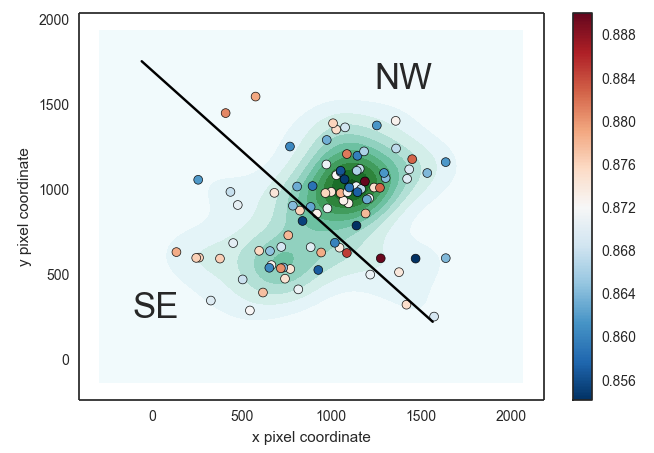
\includegraphics[width = \linewidth]{confirmed_member_divide.png}
	\caption{\label{fig:membership} Points showing the locations of the
	member galaxies and the division of the member galaxies among the two subclusters of El Gordo by a spatial cut
(black line). The color of the points shows the corresponding spectroscopic
redshift of the member galaxies (see color bar for matching of
spectroscopic values), with the redder end indicating higher
redshift. The background number density contours in green indicate a bimodal
distribution.} 
\end{figure}

%-----------------------------------------------------------------------
\subsubsection{Weak lensing mass estimation} 
%
%The input 
We obtained the PDFs of the masses of the subclusters by doing a Monte
Carlo Markov Chain (MCMC) analysis of the reduced shear from the
weakly lensed background galaxies similar to \citet{Dawson12}. We computed the reduced shear signal
generated by two NFW halos according to \citet{Umetsu10} (See Appendix
\ref{app:MCMC} for
details of implementation and output diagnostics).
At each step we followed the procedure of a
Metropolis algorithm.  The transition kernel was set to
be the log likelihood of fit of the model shear to the reduced shear of the
data (\ref{eqn:jointposterior}).
In total, eight MCMC chains were used. After every 5000 MCMC steps for all
the chains, we computed the R coefficient \citep{Gelman92}  to
check for convergence. We performed more MCMC steps as long as convergence
was not achieved. After convergence was achieved, we removed the
burn-in portions of the MCMC chains and used the resulting MCMC chains as
samples of the PDFs of the masses. \par 
% this is from Jee13 section 3.5
We make use of an effective redshift of $z_{\text{eff}} = 1.37$ or $\beta
= 0.276$ \citepalias{Jee13} and $g' \approx (1 + 0.79 \kappa)~g$ \citepalias{Jee13}
and \citep{Seitz97}.    
%\textbf{The inputs of our MCMC mass inference are from proposal blah,
%which is similar to \citepalias{Jee13}, however, this
%separate implementation of the MCMC analysis code is different than
%\citepalias{Jee13}.} 
We used a catalog of reduced and bias-corrected background 
galaxy shapes from Hubble Space Telescope PROP 12755, and these galaxies
were discussed as the population in Region A in
\citetalias{Jee13}. (! \citealt{Jee13} actually used
additional data) On the other hand, we fixed the
position of the centers of the NFW halos to be  the luminosity peaks of the
respective galaxy populations of  the two subclusters, which are at R.A. $=
01$:02:51.68, Decl. = $-49$:15:04.40 and R.A. = $01$:02:38.38, Decl. =
$-49$:16:37.64 for the NW and SE subclusters
respectively \citepalias{Jee13}. (! Lori and Nick actually asked why we do not free
the centroids like Jee 13)  The agreement between our analysis and \citepalias{Jee13} to within
the 68\% credible interval serves as a sanity check on the estimated masses. 
%Other sanity check including the control of acceptance rate between 20\%
%and 50\%. 

The mass estimates from \citealt{Jee13} are $M_{200c} = 13.8 \pm
2.2 \times 10^{14}~h_{70}^{-1} M_{\sun}$ for the NW subcluster and $ M_{200c} = 7.8 \pm
2.0 \times 10^{14}~h_{70}^{-1} M_{\sun}$ for the SE subcluster. 

We obtained 40, 000 samples of the joint PDFs of the masses of the two dark
matter halos as the outputs of the Monte Carlo Markov Chain (MCMC)
procedure from \citealt{Jee13}. Discussion of the handling of the weak
lensing source galaxies and the details the MCMC procedure for mass
estimation can be found in \citealt{Jee13}. 

%----------------------------------------------------------------------

\subsubsection{Estimation of projected separation ($d_{proj}$)} 
To be consistent with our MCMC mass inference, our Monte Carlo simulation takes 
the projected separation of the NFW halos to be those of the inferred
DM centroid locations in \citealt{Jee13}. We draw random samples
 of the location of centroids from two 2D Gaussians centered at
 RA=01:02:50.601, Decl.=-49:15:04.48 for the NW subcluster and RA =
 01:02:56.312, Decl. = -49:16:23.15 for the SE
subcluster, with a 1'' standard deviation each. Or equivalently, the
samples of the inferred centroid locations correspond to a projected separation of
$0.74\pm {0.007}$ Mpc. 
%A iterative centroiding method is used to find the centers of the two
%subclusters of El Gordo.

\subsection{Outputs of the Monte Carlo simulation}\label{sec: outputs}
%We outline the outputs of the simulation here to facilitate the discussion
of the design of the priors used in the simulation. The simulation
provides PDF estimates for many of the output variables. Variables
of the most interest include the time dependence and $\alpha$, which is
defined to be the projection angle between the plane of the sky and the merger axis. Other output variables are dependent on $\alpha$ and the time
dependence. Specifically, the simulation denotes the time dependence by
providing several characteristic time-scales, including the time
elapsed between the collision and when the subclusters first reach apoapsis
($T$) and the time-since-collision.  

The two versions of the time-since-collision variables $TSC_0$ and
$TSC_1$ denotes different possible merger scenarios. 1) We call the scenario for which the subclusters are
moving apart after collision to be ``outgoing" and it corresponds to the
smaller $TSC_0$ value, and 2) we call the alternative scenario 
``returning" for which the subclusters are approaching each other after turning
around from the apoapsis for the first time and it corresponds to $TSC_1$.
We describe how we use to break the degeneracies of the two scenarios in
section \ref{sec: positionprior}. 
 
The simulation also output estimates of variables that characterize
the dynamics of the merger. The 3D velocities, both at the time of the
collision ($v_{3D}(t_{col})$) and at the time of observation
($v_{3D}(t_{obs})$) are provided. The maximum 3D separation ($d_{max}$),
which is defined to be the distance between the position of collision to
the apoapsis, is also part of
the outputs. (See the lower half of Table \ref{tab:outputs} for all the outputs).
%Here we present results based on:\\  %1) a flat radio prior\\
%2) a uniform prior over a range of most likely 3D separations\\
%3) a Gaussian prior  
%We discuss in subsection \ref{sec:priors}  on the use of the default filters
%and two new filters designed according to the observed data and the physics of the radio relic.
%
%\textbf{While the underlying formalism of the Monte Carlo simulation is
%    based on the Bayes theorem, we caution the reader that this simulation
%    does not correspond to a conventional Bayesian parameter estimation but
%    more similar to the Bayesian uncertainty estimation method mentioned in Saltelli 
%    et al. (2004). (See appendix \ref{} for a more in-depth discussion)}



We outline the outputs of the simulation here to facilitate the discussion
of the design of the priors used in the simulation. The simulation
provides PDF estimates for 8 output variables. Variables
of the most interest include the time dependence and the angle $\alpha$, which is
defined to be the projection angle between the plane of the sky and the merger axis. Other output variables are dependent on $\alpha$ and the time
dependence. Specifically, the simulation denotes the time dependence by
providing several characteristic time-scales, including the time
elapsed between consecutive collisions
($T$) and the time-since-collision of the observed state (TSC).  

We provide two versions of the time-since-collision variables $TSC_0$ and
$TSC_1$ to denote different possible merger scenarios. 1) We call the scenario for which the subclusters are
moving apart after collision to be ``outgoing" and it corresponds to the
smaller $TSC_0$ value, and 2) we call the alternative scenario 
``returning" for which the subclusters are approaching each other after turning
around from the apoapsis for the first time and it corresponds to $TSC_1$.
We describe how we make use of properties of the radio relic to evalute
which scenario is more likely in
section~\ref{sec: positionprior}. Evolution of the merger after the second
passage is not considered.
 
The simulation also output estimates of variables that describe
the dynamics and the characteristic distances of the merger. The relative
3D velocities of the subclusters, both at the time of the
collision ($v_{3D}(t_{col})$) and at the time of observation
($v_{3D}(t_{obs})$) are provided. The characteristic
distances included in the outputs are the maximum 3D separation ($d_{max}$),
which is the distance between the position of collision to
the apoapsis and the 3D separation of the subclusters at observation
($d_{3D}$). 
%-----------------------------------------------------------------------
\subsection{Design and application of priors} 
\label{sec:priors}
%The strength of the Monte Carlo simulation by \citep(D13) is its ability
to detect and rule out extreme input values that would result in
unphysical realizations. 
Our default Monte Carlo filters are described in D13 and they are applied to ensure 
unphysical realizations in the simulation are ruled out. 
In addition to the default filters, we also examine the effects of applying 
two filters derived based on the position and the integrated polarization
fraction of the radio relic of El Gordo respectively. 
%(See Appendix \ref{tab:priors} for a complete list of filters used in this paper.) 

\textbf{El Gordo shows remarkable double radio relics on the periphery
(M11)} The radio relic  of El Gordo was first mentioned in the Sydney University
Molonglo Sky Survey (SUMSS) data in low resolution at 843 MHz
\cite{Mauch03} as shown in
M11. The higher resolution radio observation conducted by \cite{L13} at 610
\mega Hz and 2.1 \giga Hz confirms that those radio emission correspond to
radio relic after removing effects of radio point sources.
%\begin{itemize}
%\item talks about the observable, which is the comoving kinetic power through each shock surface
%\item refer to diffussive shock acceleration (DSA) mechanism?
%\item Kang \& Jones treatment of Mach number-dependent efficiency
%considering the possibility of having an non-isotropic magnetic field  
%$KJ_BparallelRadial$ model
%\end{itemize}

Radio relics have been suggested to be able to constrain the
mass ratios, the projection and the merger configuration. (Cite one of Reinout's paper) 
Ever since the first detection of radio relic,cosmological hydrodynamical simulations of
merging clusters have been used to model their emission spectrum and
geometry. (Vazza et al. 2011, van Weeren and Bruggen 2011 et al., Bonafede
et al. 2013, En{\ss}lin et al. 1997, Br\"{u}ggen et al.,  Skillman et al.
2013) While such cosmological simulations have provided valuable insights
to verifying the physical models, they are expensive both in terms of
computational power and novel techniques have to be invented in order to
analyze the large amount of simulated data so progress has been slow. 
Our Monte Carlo simulation can make use of known physics combined with the
preliminary results from such cosmological simulations to use properties of
the radio relic to constrain merger dynamics. 
Compared to hydrodynamical simulations or cosmological simulations, this
    Monte Carlo simulation is not demanding in terms of CPU time, therefore, we
    can run many realizations in order to probe how the input variables
affect the output variables. 

%\begin{figure}
%	\includegraphics[width=\linewidth]{d_3d_prior1.png}
%	\caption{The marginalized output PDFs of the observed 3D separation
%		($d_{3D}$) 
%		with and without the radio prior applied. 
%		(maybe I should replot this more nicely without too many
%		distracting lines but only the lines showing the location)
%		%The vertical
%		%lines denote, dashed line: biweight location, dash-dot
%		%line: 68\% credible limit, dotted line: 95\% credible
%		%limit.
%	\label{fig:radioprior}}
%\end{figure}


%\subsubsection{Weighting function based on the observed position of the radio relic}\label{sec:relic} 
%-----------------------------------------------------------------------
%Among the known galaxy cluster mergers that are associated with radio
%relics, \cite{Vazza12} noted that most of them have radio relic located
%more than 800 \kilo pc away from the merger center. \cite{Vazza12} then
%conducted hydrodynamical simulations of twenty of known galaxy mergers with 
%radio relic to investigate this observed trend. They found a radial
%trend of kinetic power dissipation increasing up to around half the virial
%radius (r$_{vir}$) of the cluster. Summarizing the results from the proposed model for energy dissipation of the radio relic, \cite{Vazza12} gives the range of highest kinetic power emission in a range of 
%$.2 ~r_{\mathrm{vir}} < d_{\mathrm{3D}} < .5~r_{\mathrm{vir}}$.
%
%
%% In particular, Vazza et al. (2011) showed dependence of observed
%%location of radio relic: when the clusters are at small separation, the
%%Mach number is too high for a radio shock to form and the steep fall off of
%%the emission power of the radio relic as a function of separation makes it
%%difficult to observe a radio relic when it has propagated beyond a certain
%%separation.  
%
%%\textbf{We take into account the uncertainties of their modeling and 
%% construct prior probability on a range of 3D separation for which the kinetic
%%power dissipation of the radio relic is more than 10\% of the peak value.} 
%Since we do not have information on how the probability of
%being able to observe the relic would fall off as a function of emission power, we adopt a conservative approach and designed a uniform prior. 
%%and contrast that to a flat prior to test the effect of the prior on the output variables. 
%We also take into account the uncertainties of the different proposed power
%emission model and come up with a prior of:
%\[
% \text{P}({d_{3D}}) = 
%\begin{cases} 
%\text{constant,} & \text{for 1.0  Mpc} < d_{3D}(t_{\mathrm{obs}}) < 3.0 \text{ Mpc}\\
%0, & \text{otherwise}
%\end{cases}
%\]
% for El Gordo.\par 
%%\begin{equation}  
%%P(d_{3D}(t_{\mathrm{obs}})) = 
%%\begin{cases}
%%1/C, \text{ if }1.0 \text{ Mpc } < d_{3D}(t_{\mathrm{obs}}) < 3.0 \text{ Mpc} \\ 0, \text{ otherwise}
%%\end{cases}
%%\end{equation}
%
%\begin{figure}
%	\includegraphics[width=\linewidth]{alpha_pdf_prior_diff.png}
%	\caption{The projection angle with and without the radio relic
%prior applied. (Needs to update and label the figure better)} 
%\end{figure}

\begin{table*} 
\begin{minipage}{180mm} 
\caption{Table of the output PDF properties of the model variables and
output variables from Monte Carlo simulation
\label{tab:outputs}} 
\begin{tabular}{@{}lccccccc@{}}
\toprule 
&&&Default priors & & &Default + position priors  \\ 
\hline
Variables & Units & Location & 68$\%$ CI $^{\dagger}$ & 95$\%$ 
CI & Location & 68$\%$ CI  & 95$\%$ CI \\
\hline
$\alpha$ &(degree)&&&&&&\\ 
\hline
$TSC_0$&Gyr&&&&&&\\
$TSC_1$&Gyr&&&&&&\\
$T$&Gyr&&&&&&\\
$d_{max}$ &Mpc&&&&&&\\
$v_{3D}(t_{obs})$ & \kilo \meter~\second$^{-1}$ &&&&&&\\
$v_{3D}(t_{col})$ & \kilo \meter~\second$^{-1}$ &&&&&&\\
$d_{max}$ &Mpc&&&&&&\\
$d_{3D}$ &Mpc&&&&&&\\
\bottomrule 
\end{tabular} 
\footnotesize{\\$\dagger$ CI stands for credible interval} \\ 
\end{minipage} 
\end{table*} 

One of the biggest strengths of the Monte Carlo simulation by \citetalias{D13} is its ability
to detect and rule out extreme input values that would result in
unphysical realizations via the application of prior probability. 
Our default priors are described in D13 and we include them in Appendix~\ref{app: results} for the convenience of the readers. 
In addition, we have come up with a prior on the projection angle $\alpha$
based on the polarization fraction of the radio relic.

%---------------------------------------------------------------------------
\subsubsection{Monte Carlo prior based on the polarization fraction of the radio relic}
%In particular, \cite{L13} reports an integrated
polarization fraction of $\sim33\%$ for the two identified relics. The
high integrated polarization fraction can be explained by uniformly aligned
magnetic field. (Synchrotron emission from unorganized magnetic field are
randomly polarized) We refer to a model from \citet{E98} with
the following physical picture: during a merger, the intracluster medium is compressed, this aligns the unordered
magnetic field perpendicular to the line joining the cluster center to the
radio relic. (\citealt{E98}, \citealt{vanWeeren10}, \citealt{Feretti12})
Thus, the synchrotron emission emitted from the electrons near this aligned
magnetic field is strongly polarized perpendicular to this magnetic field. \par
\textbf{The major assumption behind the design of our filter
is that the integrated polarization fraction is a monotonically
decreasing function of $\alpha$.} 
This assumption is inspired by the class of models given by \cite{E98}, 
which, despite various inputs for spectral indices and magnetic field strength, each predicts a monotonically decreasing integrated
polarization fraction as a function of $\alpha$. 
%This assumption is yet to be verified by cosmological simulations of radio relic. 
In particular, we refer to a model from \cite{E98} that would give the most
conservative estimate on the upper bound of $\alpha$. 
This model predicts a maximum integrated polarization fraction of
$\sim75\%$ when $\alpha = 0$ . From this model, the observed integrated
polarization fraction of 33\% corresponds to $\mu_\alpha =  39\degree$. 
%We consider 39\degree as an upper bound on the projection angle since this idealized model assume isotropic distribution of magnetic field and
%electrons. 
This  polarization fraction of $\sim 75\%$ predicted by \citep{E98} is
consistent with the upper bound of relic polarization fraction in cosmological
simulations \citep{S13}. No other model of the magnetic field should predict a higher polarization fraction, thus it is highly unlikely that we see 33\%
integrated polarization at $\alpha > 39\degree$. \par 
\textbf{We cannot rule out $\alpha \leq 39\degree$ as a result of possible
variations in the magnetic field.} \cite{E98} assumes an isotropic
distribution of electrons in an isotropic magnetic field. Cosmological
simulations of radio relics from \cite{S13} show varying polarization
fraction across and along the relic assuming $\alpha = 0$, resulting in a
lower integrated polarization fraction. 
%Due to these likely variations in the true magnetic field, the true observable integrated polarization values at a given $\alpha$ can be lower than what is predicted by \cite{E98}. 
%For example, it is possible that the radio relic of El Gordo has a lower maximum face-on polarization fraction than 75\%, but if we are viewing the relic at a smaller $\alpha$, the integrated
%polarization fraction can still comes out to be 33\%.
For example, it is possible to see a edge-on radio relic ($\alpha = 0$) with integrated polarization fraction of 33\%. 
\par 
%With simplifying assumptions, \cite{E98} have derived the integrated polarization fraction of a radio relic as a function of the viewing
%angle ($\delta = 90\degree - \alpha$).
% and the compression
%\~{R} of the magnetized region where the relic is generated. 
%. The simplifying assumptions, such as having an
%isotropic distribution of unshocked magnetic fields and electrons etc.,
%represents an idealized case showing maximum possible polarization fraction at a given $\alpha$.  
%% Cosmological simulations of radio
%relic \citep{S13} show a maximum integrated polarization fraction $\sim75\%$ at
%$\alpha = 0$ as predicted by \cite{E98}. 
%After accounting for different spectral
%indices and magnetic field strength, 
%The simplifying
%assumptions, such as having an isotropic distribution of unshocked fields
%and an isotropic distribution of electrons etc. \citep{E98}, gives
%polarization fraction as high as $\sim$ 75\% when $\alpha = 0$. 

%For an
%actual merger, the magnetic field can be less isotropic,  and the resulting polarization fraction at a given $\alpha$ would be lower. This postulate is backed up by the edge-on view of polarization fraction of simulated relics, such as the top left hand panel of figure 9 from Skillman et al. 2013.
%%This model, however, assumes an isotropic distribution of electrons in an isotropic magnetic field. \cite{E98}
%%These mathematical relationships underlies the design of this prior based on observed polarization fraction. The different cases that \cite{E98} considered have different magnetic field strengths and various spectral indices.
%We note that power of polarized synchrotron emission from relativistic electrons has a ratio of 7:1 between parallel polarization and perpendicular polarization. 
%Therefore,   
%
%\par
\textbf{Observation also introduces uncertainties that we have to take into account}. \cite{S13} shows that after convolving the
simulated polarization signal with a Gaussian kernel of 4\arcmin to match
observable resolution, the polarization fraction drops to between 30\% to
65\% even when $\alpha = 0$. 
Other uncertainties come from the fact that the inferred spectral indices
differ between the two observed frequencies and vary between the three
identified relic sources \citep{L13}. 
%\textbf{We pick a form of uniform prior, to represent
%the uncertainties in both the modeling (\citealt{E98}, \citealt{S13}) and the interpretation of the data from \cite{L13}.} 
Following previous discussion, we pick a value of $\mu_\alpha =39\degree +
2 \degree$ to filter realizations, i.e. we do not draw values of $\alpha >
41\degree$. The extra $2 \degree$ in the prior is included to account for the uncertainty of the integrated polarization fraction reported by \cite{L13}. 

%For the width of fall off of the sigmoidal function, we pick
%$\sigma_\alpha = 1\degree$ that corresponds to the uncertainty of the
%integrated polarization fraction reported by \cite{L13}.    

%\begin{itemize}
%\item spectral index of ...
%\item During the merger process, the hot intracluster is cluster merger compresses the magnetic field and orders the polarization.    
%\item \cite{L13} reported that the polarization can constrain viewing angle to be $> 18 \degree $-- check if this viewing angle is defined the same way 
%\item Ensslin 's work which is an application of the theory of
%plane-parallel shock acceleration, which can be justified by the large
%radius of the shock sphere
%\item we consider the most conservative constraint that can be recovered
%from this model, which is strong/weak field case with a spectral index of
%$\alpha_{\text{spectral}}\sim 2$ combined with the observed mean
%polarization fraction of $P \sim 33.3\%$, we recover a  
%\item
%\end{itemize}
%\begin{equation}
%P(\alpha) = 
%\frac{1}{2} - \frac{1}{2} \text{erf}\left(\frac{1}{\sqrt{2}}\frac{\alpha -
%(\mu_\alpha+3\degree)}{\sigma_\alpha}\right)  
%\label{eqn:prior}
%\end{equation}
%
%\noindent See Appendix \ref{app:priors} for a plot of (\ref{eqn:prior}).

%The polarization information has larger constraining power than the .   
%To test the effects of applying the prior on the aforementioned range of
%separation,  we have come up two priors and applied them separately
%%Therefore, the distance between the subclusters, which has to be less than twice the 3D distance between the radio relic from the center of the cluster, is taken conservatively to be $1.0~\mega$pc $<$ d$_{\mathrm{3D}}
%%(t_{\mathrm{obs}}) < 3.0~\mega$pc. 
% to the 3D separation of the subclusters at the time of observation 
%($d_{\mathrm{3D}}(t_{\mathrm{obs}})$):
%
%The effect of the uniform prior is shown in Figure \ref{fig:radioprior}.
%
%%\textbf{description of the radio observation} 
%
%\textbf{how the distances were determined - overview of previous work}
%


We can relate the polarization fraction of the radio relic to the
projection angle by examining the
generating mechanism of the radio relic.
The observed radio relic is due to synchrotron emission of free electrons in a
magnetic field. If the magnetic field is uniform, the observed
polarization fraction of the synchrotron emission of the electrons depends on the
viewing angle (or equivalently the projection angle) with respect to the alignment of the magnetic field. 
Synchrotron emission from electrons inside unorganized magnetic field are
randomly polarized. The high reported integrated polarization fraction from
\citet{L13} can be explained by a highly aligned magnetic field,
created by the compressed intracluster medium during a merger
(\citealt{E98}, \citealt{vanWeeren10}, \citealt{Feretti12}).
This picture is consistent with a high polarization fraction perpendicular
to this magnetic field along the relic. 
\par
We designed our prior to reflect how $\alpha$ decreases monotonically as the
maximum observable integrated polarization fraction. 
\begin{figure}
	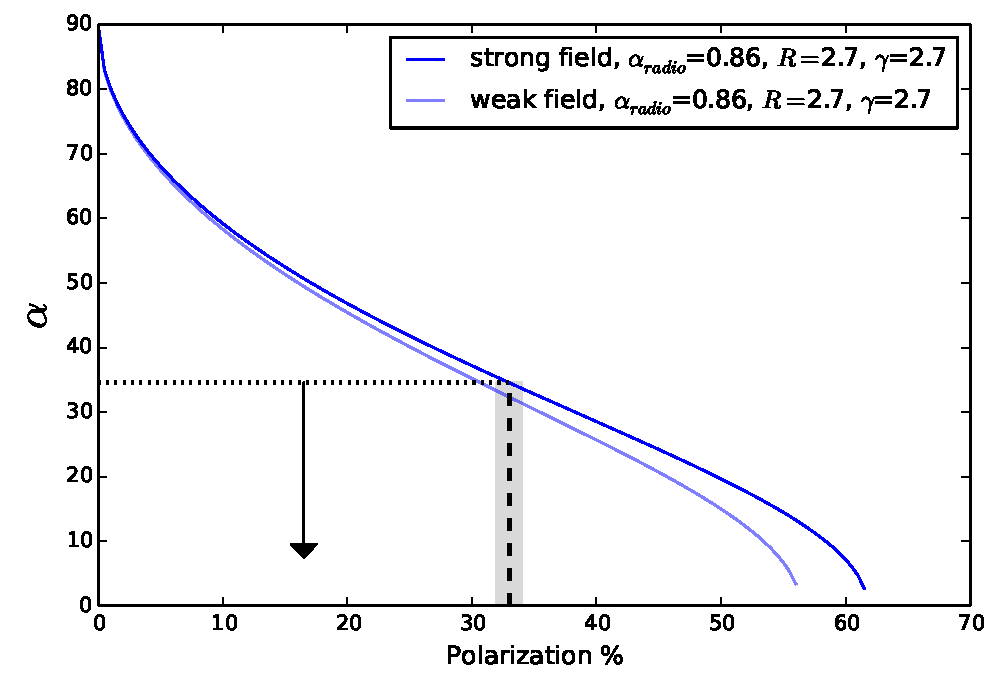
\includegraphics[width=\linewidth]{Ensslin_polar_fig.pdf}
	\caption{Predictions of polarization percentage of the radio relic at a
		given projection angle from different models, reproduced from
		\citealt{E98}. Each model assumes electrons producing the radio emission
		to be accelerated inside uniform magnetic field of various strengths ({\it strong} or {\it weak}). The curves are plotted with spectral index of the radio emission
		($\alpha_{radio}$), spectral index of the electrons ($\gamma$) and
		compression ratio of the magnetic field ($R$) corresponding to the
		estimated values from \citet{L13}.
		We highlight the observed polarization percentage of the main NW radio relic
		of El Gordo by the dotted vertical line with the greyed out region
		indicating the uncertainty \citep{L13}.\label{fig:Ensslin_fig}}
\end{figure}
This assumption is based on the class of models given by \cite{E98}(See
Figure~\ref{fig:Ensslin_fig}). In particular, we refer to a model from \cite{E98} that would give the most
conservative estimate on the upper bound of $\alpha$:
\begin{align}
\alpha &= 90 \degree -
\arcsin
\left(
\sqrt{
\frac{
	\frac{2}{15} \frac{13R - 7}{R - 1} \frac{\gamma + 7/3}{\gamma + 1}
	\langle P_{strong} \rangle}{
	1 + \frac{\gamma + 7/3}{ \gamma +1} \langle P_{strong} \rangle }}\right)
\end{align}

This model corresponds to the strong field case with the relic being supported by
magnetic pressure only, with $\alpha_{radio} = 0.86$, compression ratio
$R=2.7$ and $\gamma = 2.7$. 
This model predicts a maximum integrated polarization fraction of
$\sim60\%$ when $\alpha \rightarrow 0$. From this model, the observed integrated
polarization fraction of $33\%\pm1\%$ corresponds to an estimated value
of $\hat{\alpha}
 = 35\degree$. 
%We consider 39\degree as an upper bound on the projection angle since this idealized model assume isotropic distribution of magnetic field and
%electrons. 
This  polarization fraction of $\sim 60\%$ predicted by \citep{E98} is
consistent with the upper bound of relic polarization fraction in cosmological
simulations \citep{S13}. No other model of the magnetic field should predict a higher polarization fraction, thus it is highly unlikely that we see 33\%
integrated polarization at $\alpha > 35\degree$.  
\par

We cannot rule out $\alpha \leq 35\degree$ as a result of possible
variations in the magnetic field. 
\cite{E98} assumes an isotropic distribution of electrons in an isotropic magnetic field. Cosmological
simulations of radio relics from \cite{S13} show varying polarization
fraction across and along the relic assuming $\alpha = 0$, resulting in a
lower integrated polarization fraction. For example, it is possible to see a edge-on radio relic ($\alpha = 0$) with integrated polarization fraction of 33\%. 
Furthermore, \cite{S13} shows that after convolving the
simulated polarization signal with a Gaussian kernel of 4\arcmin~to
illustrate effects of non-zero beam size, the polarization fraction drops to between 30\% to
65\% even when $\alpha = 0$. We examined the effects of perturbing
the cutoff value of this prior to ensure the uncertainties do not
introduce significant bias in the estimated output variables and we
present the results in Appendix \ref{app: results}.
To summarize, we adopt a conservative uniform prior to encapsulate the
information from the polarization fraction of the radio relic as:
\begin{equation}
P(\alpha) = 
	\begin{cases}
	& \text{const. $>$ 0 for  }\alpha < 35 \degree \\ 
	& 0 \text{ otherwise}\label{eqn: polarprior}
	\end{cases}
\end{equation}

We refer to \ref{eqn: polarprior} as the polarization prior. Unless
otherwise stated, the main results of the paper are obtained after applying
this polarization prior in addition to the default priors.

%---------------------------------------------------------------------------
\subsection{Extension to the Monte Carlo simulation - Determining merger
scenario with radio relic position by model comparison}
%\begin{figure} 
%	\includegraphics[width =\linewidth]{shock_evolution.pdf}
%	\caption{The simplified view of time evolution of the speeds of the
%	different cluster components during the collision. }
%\end{figure}
%\label{sec: positionprior}
%% this line is included when individual section needs to be compiled and
% reviewed  
%% mn2esample.tex
%
% v2.1 released 22nd May 2002 (G. Hutton)
%
% The mnsample.tex file has been amended to highlight the proper use of
% LaTeX2e code with the class file and using natbib cross-referencing.
% These changes do not reflect the original paper by A. V. Raveendran.
%
% Previous versions of this sample document were compatible with the LaTeX
% 2.09 style file mn.sty v1.2 released 5th September 1994 (M. Reed) v1.1
% released 18th July 1994 v1.0 released 28th January 1994

\documentclass[letterpaper,useAMS,usenatbib]{"mn2e"}
%\documentclass[letterpaper,useAMS]{"mn2e"}
%LINUX version of the path
%\documentclass[useAMS,usenatbib,letterpaper]{"/media/blank/Macintosh
%HD/Users/karenyng/Library/texmf/tex/latex/commonstuff/mn2e"}

% If your system does not have the AMS fonts version 2.0 installed, then
% remove the useAMS option.
%
% useAMS allows you to obtain upright Greek characters.  e.g. \umu, \upi
% etc.  See the section on "Upright Greek characters" in this guide for
% further information.
%
% If you are using AMS 2.0 fonts, bold math letters/symbols are available
% at a larger range of sizes for NFSS release 1 and 2 (using \boldmath or
% preferably \bmath).
%
% The usenatbib command allows the use of Patrick Daly's natbib.sty for
% cross-referencing.
%
% If you wish to typeset the paper in Times font (if you do not have the
% PostScript Type 1 Computer Modern fonts you will need to do this to get
% smoother fonts in a PDF file) then uncomment the next line 
%\usepackage{Times}

%%%%% AUTHORS - PLACE YOUR OWN MACROS HERE %%%%%
\usepackage{hyperref}
\usepackage{amssymb}
\usepackage{graphicx}
\usepackage{amsmath}
\usepackage[amssymb]{SIunits} 
\usepackage{booktabs}
\usepackage{hhline}
\usepackage{breqn}
\usepackage{standalone}
\usepackage{dcolumn}
	\newcolumntype{d}[1]{D{.}{.}{#1}}
\usepackage{tabularx}
\usepackage{booktabs}
\graphicspath{{graphics/}}
\newcommand{\mc}[1]{\multicolumn{1}{c}{#1}} % handy shortcut macro
%-----------------------------------------------------------------------

%\begin{document}

% draft: 
% explain that 4300 km /s from L13 
% explain how the position of the radio relic is calculated 
% explain the physics / concepts behind this calculation 
% explain the assumptions
% explain the data 
% decide on which frame of reference we want to do the calculation in 
% corresponding code: position_prior_elgordo.ipnb in
% TSM/mercury_elGo/Feb_data folder 
% incorporate the uncertainty of the centroid position???????
% paragraph 1: explain where the data comes from and how they are used 
% why only the NW relic is used but not the SE one ?
%Even though there is a list of standard required data as denoted in section
%\ref{sec: inputs} for the simulation, it is straight forward to incorporate
%new data variables. 
%With additional of data from the radio relic
%\citep{L13}, this simulation is capable of providing a quantitative view of
%how likely each of  the two possible merger scenarios mentioned in section
%\ref{sec: outputs} is true. 
%We make reference to the radio relic data from \cite{L13} in this
%subsection for extending the simulation. Three sources of radio relic
%were identified - including the NW, SE and the E relic. The NW radio
%relic possesses the most extended geometry among all the identified relic source. 
%
%% make sure of Springel and Farrar 
%% the frame of the shock given by Lindner et al. is complicated 
%% there is no trivial translation between  
%We do not refer to the The SE nor the E radio relic in this calculation
%since we do not have an estimation of the shock speed of the SE relic
%nor the E relic from \citealt{L13}.    
%We incorporate the calculated shock speed of the radio relic as part of
%$\vec{D}$ for the Monte Carlo simulation. 
%We draw  $v_{relic} \sim N(4300~\kilo\meter~\second^{-1},
%800~\kilo\meter~\second^{-1})$ \citep{L13} from each realization and
%compute how far the NW relic would have traveled given a certain TSC in the
%frame of the SE subcluster. Finally we compare the distance traveled
%predicted from the simulation to the reported position of the NW relic at RA = 01:02:46, DEC = -49:14:43\citep{L13}.
%
% this paragraph should really discuss why we are assuming constant speed 
% paragraph 2: estimate the upper and lower bound of the speeds and how
% that is going to impact the conclusion drawn 
% Ambiguity about the speed:
% do we need to talk about that we are only referring to the NW relic not
% the SE relic? Yes! 
% do we need to explain why we are only using the NW relic not the SE
% relic?
We give constraints on the likelihood of the
outgoing and returning merger scenarios by comparing the observed and the
simulated position of the NW radio relic.
This method depends on the estimate of the
time evolution of the relic velocity, which gives the upper and lower
bounds on the possible position of the relic for each scenario. The
velocity depends on a number of physical quantities, including the
local gravitational potential, matter density, temperature, pressure among
others (\citealt{E98}, Shu .F., more citations?).  The exact time evolution
of the shock velocity requires detailed numerical simulation similar to
\citet{Springel2007}, \citet{Vazza11}, \citet{Kang2007}, etc.  
We considered different possibilities of the time evolution of the shock
velocity since numerical simulation of the shock of El Gordo is not
available at the time of writing of this paper. We drew physical insight from the simulations of the merger shock of the
staged numerical simulation of the Bullet cluster from \citet{Springel2007}
and the cosmological simulation from \citet{Paul2011b}. Right after
the collision of the subclusters, \citet{Springel2007} shows that the shock speed is
comparable to the merger speed of the two subclusters; the shock speed
dropped only by $\sim 14\%$ in the $300~\mega$yr period while the speed of
the main subcluster in the simulation dropped by $\sim65\%$ in the center
of mass frame. On the other hand, \citet{Paul2011b} showed that the shock
speed was $\sim1.5$ times the relative collisional speed of the subcluster
shortly after the collision and the shock speed decreases only
slightly as it propagates away from the center of mass. \par  
We approximated the upper and lower bounds of the NW relic speed with the
simulated speeds of the NW subcluster.  We simplified the calculation by
working in the center of mass frame where the shock speed is expected to
drop slightly with time. 
The projected separation of the shock is approximated as:
\begin{equation}
	s_{proj} = \langle v_{relic} \rangle (\hat{t}_{obs} - \hat{t}_{col}) \cos(\hat{\alpha})
	\label{eqn: projectedsep}
\end{equation}
where the quantities with hats on the right hand side of the equations were
inferred from the simulation, and $s_{proj}$ is the estimated projected separation and we estimated the
upper and lower bounds of the time-averaged velocity
$\langle v_{relic} \rangle$ of the shock between
the collision of the subclusters and the observed time as:  
\begin{equation}
	\langle v_{relic} \rangle = \beta~v_{3D,1}(t_{col})  
\end{equation}
where $0.8 \leq \beta \leq 1.2$ is a factor that we introduce to represent the
uncertainty of the speed of the relic and $v_{3D,1}(t_{col})$ refers to the collisional velocity of
the NW relic in the center-of-mass frame. The upper bound can be
approximated as the collisional speed of the NW subclusters due to how the
shock is powered by the collision. After the collision, it is unlikely that
there would be significant energy injected into the shock to speed up the
shock such that the shock travels much faster than the collision speed of the subcluster. While the shock does not experience gravitational deceleration as a
pressure wave, some dissipative processes may have slowed down the shock
wave slightly as it propagated. By making use of a
range of $\beta$ values, we examine how the rate of slow down would
give a different lower bound of the projected separation of the relic.   

%We compare the bounds with the observed position of the NW relic  at RA =
%01:02:46, Decl. = $-49$:14:43 \citep{L13}.
%Three sources of radio relic were identified, including the NW, SE and the
%E relic. The NW radio relic possesses the most extended geometry among all
%the identified relic source. We do not refer to the The SE nor the E radio
%relic in this calculation since we do not have an estimation of the shock
%speed of the SE relic nor the E relic from \citealt{L13} for comparison.    


%We incorporate the calculated shock speed of the radio relic as part of
%$\vec{D}$ for the Monte Carlo simulation. 
%We draw  $v_{relic} \sim N(4300~\kilo\meter~\second^{-1},
%800~\kilo\meter~\second^{-1})$ \citep{L13} from each realization and
%compute how far the NW relic would have traveled given a certain TSC in the
%frame of the SE subcluster. Finally we compare the distance traveled
%predicted from the simulation to the reported position of the NW relic 

% make sure of Springel and Farrar 
% the frame of the shock given by Lindner et al. is complicated 
% there is no trivial translation between  

%Observationally, studies from Lindner et al. also provide some
%comparison of the estimated shock speed relative to the gas medium as $4300
%\pm^{800}_{500} \kilo \meter~\second^{-1}$. 

%We simplified the computation of the position of the relic by estimating
%the time-averaged velocity of the relic.
%We treated the lower bound of the time-average
%relic velocity $\hat{v}_{relic} \approx  \hat{v}_{3D}(t_{col})$ due to how
%shock speed evolves over time.  

%We performed two sets of calculation to bracket the possible positions of
%the radio relic.
%
%%* shock speed from Lindner et al. is in the frame of  
%
%In order to capture the major uncertainty in the time evolution of the
%shock, we approximated the time-averaged velocity of the shock with a mean
%as the relative merger speed, and assumed a very wide support of $\kilo
%\meter~\second^{-1}$.
%(See Figure to denote how the distribution compares with the
%relative velocity, the observed shock velocity in the unknown frame)
%\begin{itemize}
%\item ``In previous work, it has been assumed that the shock
%			velocity is equal to
%			the subclustre's relative velocity with respect to the parent
%			cluster
%			(Markevitch et al. 2002, Hayashi \& White 2006, Markevitch
%			2006, among
%			others')'' all velocities are quoted in the CM frame
%
%\item Shock speed related to the local density / temperature / pressure of
%	the medium.
%\end{itemize}

%We denoted the speed in the SE subcluster frame, we take into consideration
%that after the collision, the SE subcluster move away from the NW
%shock(relic) at a deceleration due to the gravitational pull of the NW subcluster.
%Therefore, in the SE subcluster frame, the shock would also slow down. 
%(See figure \ref{fig:shock_evo} for the evolution of the shock wave speed
%in different reference frames)
%The study of the radio relic from \citealt{L13} also shows that the shock
%speed can be consistent with the merger speed. 
%However, since the shock speed was measured with respect to the 
%(See figure X for a distribution
%of the merger speed and how that compares to the observed relic speed) 
%
%The greatest uncertainty remains in the modeling of the time evolution of
%the speed of the shock wave.
\par      
%\bibliographystyle{mn2e}
%\bibliography{bib}
%
%\end{document}


One of the biggest question involving the merger is if El Gordo was
observed to be in a returning or outgoing phase.
We performed a Bayesian model comparison of the observed and the
simulated position of the NW radio relic in each scenario.
We considered different possibilities of the time evolution of the merger shock
.  We drew physical insight from the
simulations of the merger shock of the cosmological simulation from
\citet{Paul2011b} and a similar cluster merger of CIZA J2242.8+5301
\citep{VanWeerenRJ2011}. 
Right after the collision of the subclusters, both \citet{Paul2011b} and
\citet{VanWeerenRJ2011} showed that
merger shock fronts that may correspond to the radio relics 1) are generated
close to the center of the substructure, 2) propagated outwards with  
 the shock speed decreasing only slightly (between 10\% to 30\% via private
 communication with Paul S.) as the
 shock propagates away from the center of mass.  
\par  

Since we do not know the time-evolution of the propagation speed of the
shock front with respect to the center of mass, we express possible shock
speeds as a multiple of the inferred collisional speed of the subclusters
in the center of mass (momentum) frame, then calculate how far the shock would have propagated for our inferred
$TSC_0$ and $TSC_1$ values. We worked in the center of mass frame where the
shock speed is expected to drop slightly with TSC. 
The projected separation of the shock is approximated as:
\begin{equation}
	%s_{proj} = \langle v_{relic} \rangle (\hat{t}_{obs} - \hat{t}_{col})
	s_{proj} = \langle v_{relic} \rangle (\hat{t}_{obs} - \hat{t}_{col}) \cos(\hat{\alpha})
	\label{eqn: projectedsep}
\end{equation}
where the quantities with hats on the right hand side of the equations were
inferred from the simulation, and $s_{proj}$ is the estimated projected separation and we estimated the
upper and lower bounds of the time-averaged velocity
$\langle v_{relic} \rangle$ of the shock between
the collision of the subclusters and the observed time as:  
\begin{equation}
	\langle v_{relic} \rangle = \beta~\hat{v}_{3D,1}(t_{col})  
\end{equation}
where $0.5 \leq \beta \leq 1.5$ is a factor that we introduce to represent the
uncertainty of the velocity of the relic shockwave and $\hat{v}_{3D,1}(t_{col})$ refers to the collisional velocity of
the NW subcluster in the center-of-mass frame as a comparison. 
\label{sec: positionprior}

%the springel and farrar shock is NOT applicable to this section get rid of
%it

%This method depends on the time evolution of the relic velocity, which gives the upper and lower bounds on the possible position of the relic for each scenario. 
%%The velocity depends on a number of physical quantities, including the
%local gravitational potential, matter density, temperature, pressure among
%others (\citealt{E98}, Shu .F., more citations?).  The exact time evolution
%of the shock velocity requires detailed numerical simulation similar to
%\citet{Springel2007}, \citet{Vazza11}, \citet{Kang2007}, etc.  
%The upper bound can be
%approximated as the collisional speed of the NW subclusters due to how the
%shock is powered by the collision. After the collision, it is unlikely that
%there would be significant energy injected into the shock to speed up the
%shock such that the shock travels much faster than the collision speed of the subcluster. While the shock does not experience gravitational deceleration as a
%pressure wave, some dissipative processes may have slowed down the shock
%wave slightly as it propagated. By making use of a
%range of $\beta$ values, we examine how the rate of slow down would
%give a different lower bound of the projected separation of the relic.   
\par      

%----------------------------------------------------------------------
%\subsection{Relative merger speed}
%\input{3_overview}
%-----------------------------------------------------------------------

\begin{table*} 
\begin{minipage}{170mm} 
\caption{Table of the output PDF properties of the model variables and output variables from Monte Carlo simulation
\label{tab:outputs}}
\begin{tabularx}{\textwidth}{@{\extracolsep{\fill}}lccccccccc@{}}
\hline
\hline
&&&&Default priors & & & & Default + polarization priors  \\ 
\cmidrule{4-6} \cmidrule{8-10} 
Variables & Units && Location & 68$\%$ CI $^{\dagger}$ &95$\%$ CI && Location & 68$\%$ CI  & 95$\%$ CI \\ 
\hline 
$\alpha$ &(degree)&&43&19-69&6-80&&21&10-30&3-34\\
%$d_{proj}$ &Mpc&&0.74&0.74-0.75&0.73-0.76&&0.74&0.74-0.75&0.73-0.76\\
$d_{max}$ &Mpc&&1.2&0.9-2.2&0.77-4.6&&0.93&0.81-1.2&0.75-1.9\\
$d_{3D}$ &Mpc&&1&0.79-2.1&0.75-4.3&&0.8&0.76-0.88&0.74-0.91\\
$TSC_0$&Gyr&&0.61&0.4-0.95&0.26-2.4&&0.46&0.3-0.55&0.21-0.64\\
$TSC_1$&Gyr&&1&0.77-1.7&0.63-4.4&&0.91&0.69-1.3&0.59-2.3\\
$T$&Gyr&&1.6&1.3-2.6&1.2-7.1&&1.4&1.2-1.6&1.2-2.4\\
$v_{3D}(t_{obs})$ & \kilo \meter~\second$^{-1}$ &&580&260-1200&59-2400&&940&360-1800&62-2900\\
$v_{rad}(t_{obs})$ & \kilo \meter~\second$^{-1}$ &&360&140-630&27-880&&310&110-590&8-840\\
$v_{3D}(t_{col})$ & \kilo \meter~\second$^{-1}$ &&2800&2400-3700&2100-4200&&2400&2200-2800&2100-3500\\
\bottomrule
\end{tabularx}\\
\footnotesize{$\dagger$ CI stands for credible interval}\\
\end{minipage}
\end{table*}

\section{RESULTS} 
We found that the two subclusters collided at with a relative velocity of 
$2400\pm^{900}_{400}~\kilo\meter~\second^{-1}$, at an estimated projection
angle of $\alpha = 21\degree~\pm^{9}_{11}$. From our analysis of the two
scenarios, we found that El Gordo is more likely to be observed at a returning
phase with a estimate of $TSC_1 = 0.91\pm^{0.22}_{0.39}$ Gyr. We present an
overview of all the estimated variables in table~\ref{tab:outputs}, with
results only applying the default priors on the left hand side of the table
and those applied with the polarization prior on the right hand side.
Furthermore, we include the plots of all the marginalized PDFs with the
polarization prior in Appendix~\ref{app: results}. \par 
Our estimates of $v_{3D}(t_{col}) = 2400\pm^{900}_{400}~\kilo\meter~\second^{-1}$ at the time of collision is compatible with independent estimates from \citealt{L13}. 
By making use of the upstream velocity of the shockwave, \cite{L13}
reported an estimate of the upper bound of the relative collisional
velocity by making use of the Mach number of the NW radio relic, at $2500
\pm^{400}_{300}\kilo\meter~\second^{-1}$. Magnitude of the
relative $v_{3D}$ of the subclusters drops as the subclusters climb out of the gravitational potential of each
other, and reduced to a relative $v_{3D}(t_{obs}) = 940~\kilo\meter~\second^{-1}$ at
the time of observation. 
%Our estimate of $v_{3D}(t_{col})$ is
%also consistent with \cite{Donnert13} which made use of the same radial velocities
%of the subclusters and assumed zero initial kinetic energy.  
%With this new estimates of $v_{3D}(t_{col})$, we find that the absence of an
%X-ray bow shock feature from El Gordo, may be due to the merger speed being
%low as suggested by \citetalias{Jee13}. 


%-----------------------------------------------------------------------

\subsection{Time-since-collision (TSC) and the merger scenario}
The simulation gives two estimates for
the time-since-collision, with $TSC_0 = 0.61~\giga \text{yr}$ and $TSC_1 =
1.0~\giga\text{yr}$. Both the estimates of $TSC_0$ and $TSC_1$ are
compatible physical time-scales of observable features of El Gordo.  
Both estimates are lower than the sound crossing time of $\sim2~\giga$yr,
which an be considered for which the wake feature can be observed. 
The observable time scale of the radio relics are also on the scale of
$\sim1~\giga$yr. 

Based on section \ref{sec: positionprior}, we
present estimates for the position of the NW radio relic based on the two PDFs
of inferred TSC as shown in Fig. \ref{fig: positionprior}. We plotted
the PDF of the simulated positions of the relic for the outgoing scenario
(blue) and the returning scenario (green) against
the observed position of the relic (light red), with the width of the
relic representing the 95\% confidence interval, this uncertainty is greater than the width of the relic ($\sim$$23$
kpc) along merger axis \citep{L13}. When we
assume $\langle v_{relic} \rangle / v_{3D, 1}(t_{col}) = 1.5$ (uppermost
panel of Figure \ref{fig: positionprior}), $\langle v_{relic} \rangle$
corresponds to an time-averaged velocity of $\sim3800~\kilo
\meter~\second^{-1}$ relative to SE subcluster, or, in the center of
mass frame $\sim1400~\kilo\meter~\second^{-1}$, the outgoing scenario 
is more favored.  As we examine a decreased ratio of  $\langle v_{relic} \rangle /
v_{3D,1}(t_{col})$, we probe how much the shock could have slowed down
and still be consistent with the outgoing scenario. The second (relative
velocity of $2800~\kilo\meter~\second^{-1}$) and third row of
Fig. \ref{fig: positionprior} show that if $\langle v_{relic} \rangle
\lesssim 1.1 $, the returning scenario would be favored instead.
A definite conclusion about the best fit scenario would require better
knowledge of the time evolution of the shock velocities. 
%Estimates of \citet{L13} of the shock velocity corresponds to $2500 \pm
%^{400}_{300} \kilo \meter~\second^{-1}$, relative to the surrounding
%intracluster medium. 


%The hydrodynamical simulation of \cite{Donnert13} shows significant energy
%dissipation as their $T \approx 2 \giga $yr for the first core-passage
%dropped to $T\approx 1 \giga$ yr for the second core-passage.  



\begin{figure}
	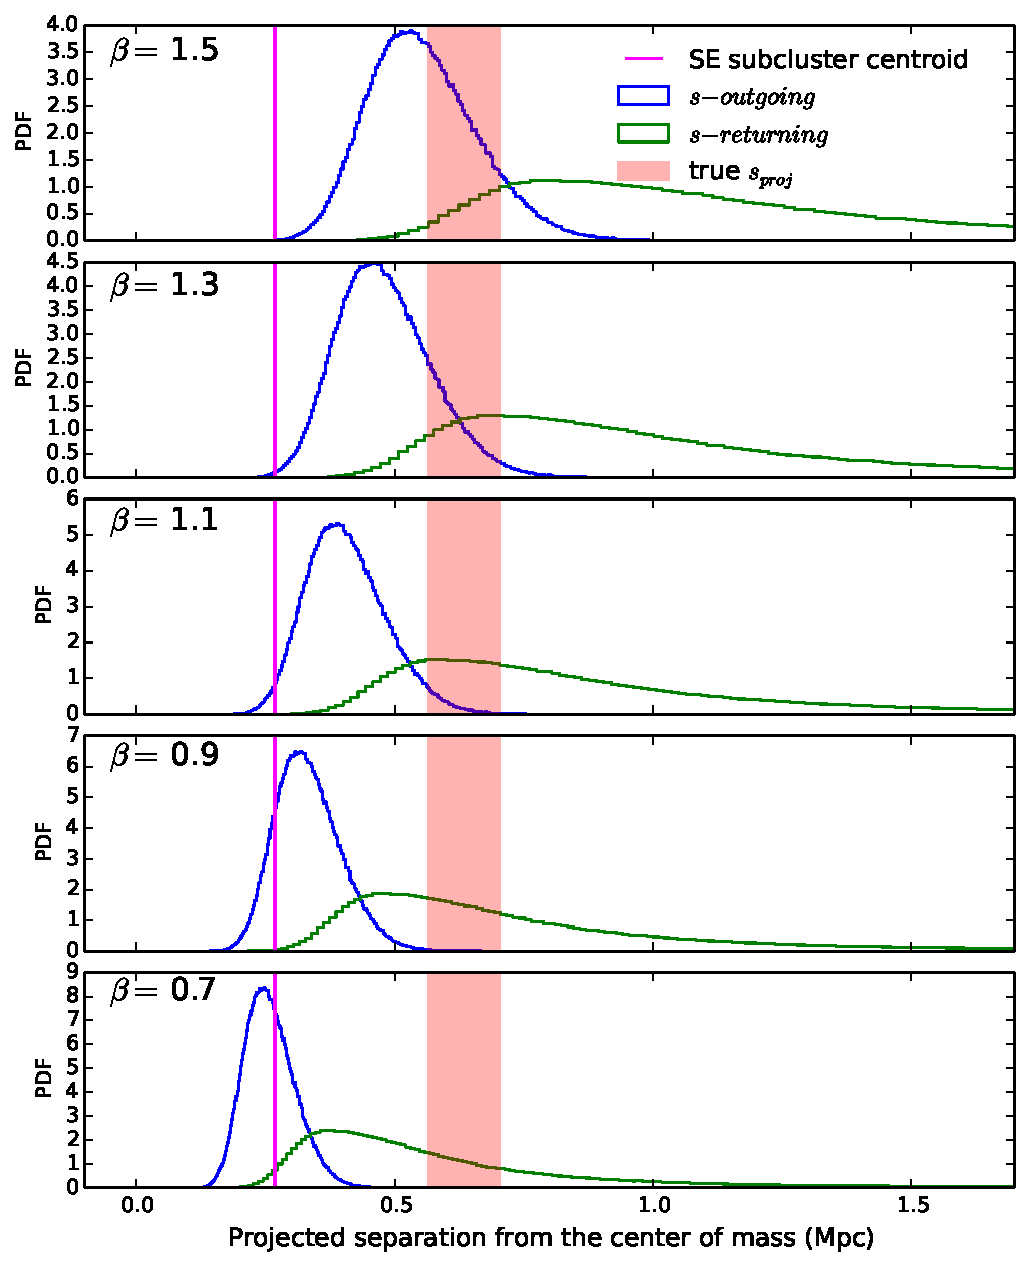
\includegraphics[width=\linewidth]{polar_prior_bounds.pdf}
	\caption{Comparison of the PDFs of the observed position of the relic (red bar
		includes 95\% confidence interval of location of relic in the center of
		mass frame) with the	predicted position from the two simulated merger scenarios (blue for
	outgoing and green for the returning scenario). We made use of the polarization prior for producing this figure. 
	\label{fig: positionprior}}
\end{figure}

\begin{figure}
	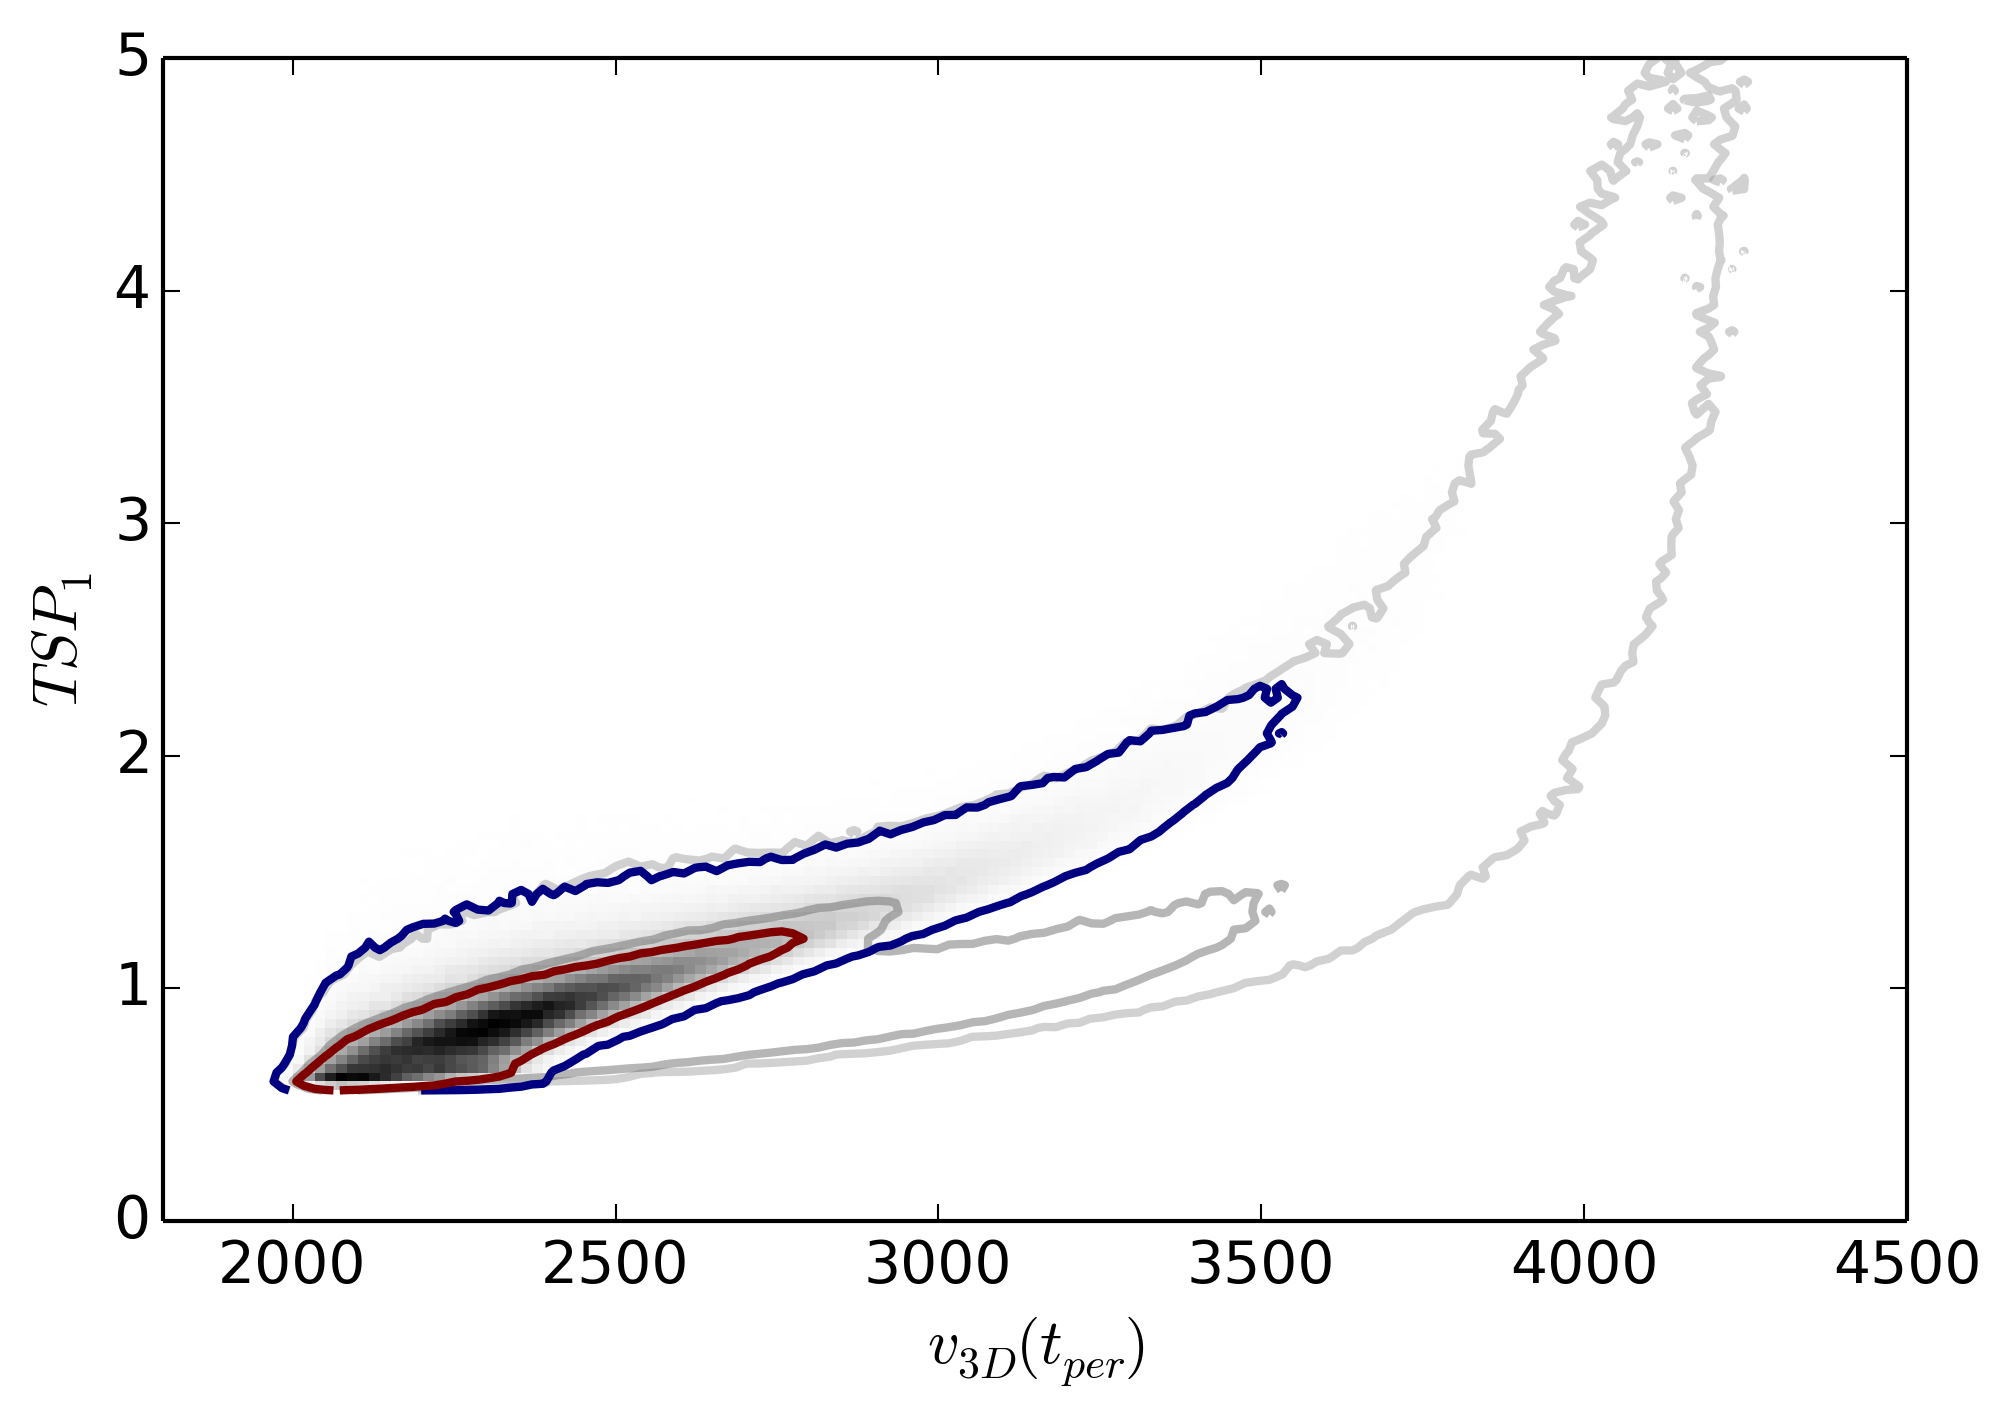
\includegraphics[width=\linewidth]{TwoMnWBSG_2contour2d.png}
	\caption{The marginalized output PDF of the returning time-since-collision
($TSC_1$) vs. the 3D velocity at the time of collision for El Gordo. The
grey set of contours show the credible regions before applying the
polarization prior and the colored contours correspond to the credible
regions after applying the priors. The contours represents the 95\% and
68\% credible regions respectively. }
	\label{fig:TSC_v3D}
\end{figure}

\subsection{Sensitivity analysis of the polarization prior}
%\label{sec: sensitivityTests}
We performed tests of how each of the output variables vary according to the
choice of the cutoff of the polarization prior between
$\alpha_{\text{cutoff}} =
29 \degree$ to $49\degree$ instead of $35 \degree$.  
We found that in the most extreme case, choosing the cutoff values as $29
\degree$ ($-6 \degree$), the location of the $v_{3D}(t_{obs})$, is
increased by $ 16 \%$. While the upper $95\%$ CI of $d_{max}$ is
the most sensitive to the prior and it changes by
$\sim 20 \%$ when $\alpha_{\text{cutoff}} = 49 \degree$. 
This shows that the exact choice of the cut off value for $\alpha$ does
not affect our estimates significantly.

%Should also talk about angle uncertainty between choosing different models
%%and how the sensitivity test show the percentage tests for those. 
%Even if we made use of the least conservative model, assuming weak field
%and a radio spectral index of 1.5 from \cite{E98}, which
%corresponds to a cutoff of $\alpha = 33\degree$, the output variable would
%be changed by X\% at most. 

%how does this affect the conclusion of our merger scenario? 
% talk about the sensitivity tests for TSM_1 and TSM_0
% talk about the sensitivity tests for  





\label{sec: sensitivityTests}
We performed tests of how each of the output variables vary according to the
choice of the cutoff of the polarization prior between
$\alpha_{\text{cutoff}} =
29 \degree$ to $49\degree$ instead of $35 \degree$.  
We found that in the most extreme case, choosing the cutoff values as $29
\degree$ ($-6 \degree$), the location of the $v_{3D}(t_{obs})$, is
increased by $ 16 \%$. While the $95\%$ CI of $d_{max}$ is
the most sensitive to the prior and it changes by
$\sim20 \%$ when $\alpha_{\text{cutoff}} = 49 \degree$. 
This shows that the exact choice of the cut off value for $\alpha$ for the
polarization prior does not change our estimates drastically.
%\subsection{Three-dimensional (3D) configuration of El Gordo}
%%\input{3.4_3D_config}
%
%The projection angle of the El Gordo is constrained by the 95\% confidence
%interval of 3 \degree and
%34 \degree, with an estimate of 21\degree.  However, we are still not taking into
%account that as $\alpha$ is increases from $65 \degree$ to $80 \degree$, the
%weak lensing estimate of the total mass of El Gordo will decrease by half.
%
%Many previous studies (van Weeren et al. CITATIONS) have suggested that
%$\alpha$ should be small for the detection of double radio relics to be
%possible but did not provide quantitative constraints.    
%
%Most of the uncertainty of the parameter estimates come from the projection
%angle as shown in Fig (X).
%Without the default priors, the Monte Carlo simulation gives the estimate
%of the projection angle as 41.7\degree, with the CI = 22.7\degree, 61.14\degree.  
%After applying the radio relic polarization prior, the CI shrinks to 
%\degree and \degree.
%Both estimates are consistent with the estimate of $\alpha > 7.8 \degree$ from
%\citet{L13} based on the dynamics of the radio relic. 
%
%More work from N-body magentodynamical simulations is needed to better understand about the physics and the
%observable contraints of
%radio relics on merger dynamics. from cosmological simulations such as,  
%More observational constraints  
%
%(More speculative stuff should be put at the end.)
%From this simulation we have shown that it is possible to detect
%the double radio relics with $\alpha$ being as big as $61.14\degree$. 
%More concrete conclusions can only be drawn with better understanding of
%the radio relic properties from simulations and observations. 
%
%Low projection angle are rejected due to the assumption of a bound system
%
%\begin{itemize}
%\item explains that there hasn't been quantitative constraints on the angle
%for which double radio relic can be observed, even though that many studies
%have suggested that the detection of radio relic should imply that $\alpha$
%should be small. 
%From this simulation we have shown that it is possible to detect
%the double radio relics with $\alpha$ being as big as $61.14\degree$. 
%
%\item James' paper did mention how the mass estimation depends on $\alpha$,
%with the estimated mass being a lot smaller if $\alpha \ge 65\degree$. 
%However, since we did use the larger mass estimate as the input of this
%simulation, we can only say that the inferred $\alpha$ is consistent with
%the mass estimation. 
%% angle dependence of observation of radio relic,  this is the first estimate 
%% that provides an upper bound on the angle
%% for which we can observe double radio relic  
%\item discussion of the different scenarios mention in M12:
%1) we are viewing after core passage, but before first turn around, and
%the merger speed is low"\\
%2) the merger speed is high, but we are viewing after the first turn
%around as the two components come together for a second core passage
%\item discuss the inclination angle estimate from M12
%\item Dave: explain where the limits of the projection angle comes
%from. what observational evidence contradicts the low velocity
%scenario the most
%\end{itemize}


\section{DISCUSSION}
%-----------------------------------------------------------------------
\subsection{Our finding in the context of other studies of El Gordo}
We outline the qualitative agreement and disagreement between our
simulations and other hydrodynamical simulations of El Gordo such as
\cite{Donnert13} and \cite{Molnar14}. Our simulation focuses on giving PDF
estimates of particular dynamical and kinematic variables, whereas the
hydrodynamical simulations focused on understanding the detailed gas dynamics
and the corresponding X-ray observables of El Gordo. The goals,
assumptions, and initial conditions of \cite{Donnert13} and \cite{Molnar14}
are different from our simulations such that detailed comparisons may not
be meaningful. 
For example, both hydrodynamical simulations were based on a few sets of initial
conditions, instead of a thorough sampling of the inputs. The outputs of
the hydrodynamical simulations are unable to convey uncertainties due to
the inputs. Both hydrodynamical simulations made use of a higher $m_{NW} =
1.9 \times 10^{15} M_{\sun}$ which is larger than the upper 95\% CI of $m_{NW}$
that we used. Furthermore, \cite{Molnar14} initialized the relative infall velocity (velocity when separation of subclusters equal the sum
of the two virial radii) to be $> 2250~\kilo \meter~
\second^{-1}$. This corresponds to $v_{3D}(t_{col}) \gtrsim 4700~\kilo
\meter~\second^{-1}$, which is close to the velocity required for the
system not to be gravitationally bound. The range of projection angles suggested by
\cite{Molnar14} of $\alpha \gtrsim 45\degree$ are also excluded by our polarization prior.  On the other hand, our simulations show qualitative agreement with
\cite{Donnert13} on the duration between consecutive core-passages. With
the time resolution of 25 $\mega$yr, the simulation from \cite{Donnert13} gave an
qualitative estimate of  $T\approx 2~\giga$yr between the first and second
core-passage in Fig. 6, while our estimate gives $T
= 1.6~\giga$yr.  A better comparison to the hydrodynamical simulations
may be achieved by performing Gaussian process emulation to obtain outputs
with more similar inputs as our simulations, but the work of fair, detailed
comparison is out of the scope of this paper. 

\subsection{Comparison to other merging clusters of galaxies}
%
Estimates of the period of El Gordo is smaller than both Musketball and
the Bullet Cluster due to the larger masses of its subclusters. 

Talks about how El Gordo is more massive and collided at higher speed than
both the Bullet and the Musketball, so El Gordo is probably a better probe of SIDM properties.

With this new piece of evidence, we find that the absence of an
X-ray shock feature from El Gordo, may not be due to the merger speed being
low, as suggested by \citetalias{Jee13}. 
In particular, taking into account that the estimated projection angle of 
$\sim 41.7\degree$, we estimate the projected relative velocity to be 597
\kilo \meter~\second$^{-1}$, which is consistent with the estimated
line-of-sight velocity differences of $586 \pm  96~\kilo \meter
~\second^{-1}$ in \citetalias{M12}. 

Furthermore, the study from \cite{L13} Lindner et al. has come up
with an estimation of the shock velocity of the radio relic of El Gordo as 
$\sim 4000~\kilo \meter~\second^{-1}$. While this shock velocity is not the
same as the merger velocity, they should be of similar magnitude. Indeed
our simulation found that a merger velocity of $4000~\kilo
\meter~\second^{-1}$ is within the 95\% credible interval. 

Dynamical properties of El Gordo are more similar to the Bullet Cluster
(cite cite)
than the Musketball Cluster (\cite{Dawson12}, \citetalias{D13}). Both the Bullet Cluster and the Musketball
were studied by \citetalias{D13} using the Monte Carlo simulation.
In addition to the default prior, \citetalias{D13} applied a temporal prior
based on the observed X-ray luminosity boost for the Bullet Cluster, while
only the default priors were suitable to be applied for the Musketball.
Therefore, with the additional priors, both the Bullet Cluster and El Gordo
show a more constrained parameter space. 
The three output variables that we compare among the listed clusters include $TSC$,
$v_{3D}$ and the masses. These variables can affect
how strongly the self-interaction of dark matter would manifest itself in
case the DM self-interaction cross section is not zero. A higher TSC might
allow more time for DM to interact with itself; a higher $v_{3D}$ might
 and a higher mass would correspond to
higher central density for a higher self-interaction rate. Although El
Gordo is the most massive among the listed clusters, the higher mass did not result in a higher $v_{3D}(t_{col})$.
The estimate of $v_{3D}(t_{col}) = 2400~\kilo\meter~\second^{-1}$ is
comparable to the inferred $v_{3D}(t_{col}) =
2800~\kilo\meter~\second^{-1}$ of the Bullet Cluster. 
Both the phase $TSC_0  \approx 40\%~T$ and the $TSC_0 = 0.6~\giga$yr are
similar between El Gordo and the Bullet Cluster
It is remained to be investigated if our hypothesis about the relationship
between how these variables would affect our chance of seeing effects from
self-interaction of dark matter. 

\subsection{Limitations of our data analysis and future work} 
We note that our method of inferring the 3D velocities by deprojecting the
radial velocities might not be optimal but is commonly used (\citetalias{M12},
\citealt{Dawson12}). The relative
radial velocities are dependent on the identification subcluster members.
However, it is unclear that a spatial
cut according to number density peaks would be optimal for selecting
galaxies that represent the underlying velocities of the subclusters. Traditionally, grouping members
may be treated as a (statistical) clustering problem with well known
methods such as normal mixture model. However, our setting is complicated
by the fact that each of the observed redshifts of galaxies is an unknown combination of cosmological redshift
and redshift due to peculiar motion along the line-of-sight. Our study
only make use of a limited number of galaxies with spectroscopy
information. This could cause selection bias and incompleteness due to
limitations of the of spectroscopic targets. Existing
literature and tests mostly focus on detecting substructures in galaxy
clusters through non-Gaussianity of the velocity dispersion (Dressler,
Einasto). Few extensive studies have focused on finding out the uncertainties
associated with this clustering procedure for inferring the dynamics of
merging clusters. This problem presents an interesting direction for investigation in the future.   
 
Despite the limitations and simplifying assumptions, this work provides
insight to the merger dynamics and configuration of El Gordo as a basis for further studies.
Tests for signs of self-interaction of DM in El Gordo  can be done
by comparing the offset between the member galaxies and the
DM distribution of the subclusters. By understanding the merging scenario,
we can infer if the observed galaxy-DM offset are in the expected
direction such that the collisionless galaxies lead the DM subhalos along
the direction of motion. In addition, our work has allowed us to examine
what information would be needed to better understanding of the merger
dynamics. Important pending questions concerning the radio relic and the
merger  include:  What are the typical propagation velocities of the shockwave that
corresponds to the radio relic in the	center of mass frame of the cluster?
What physical properties of the DM subclusters would correlate the best with the
time-evolution of the propagation velocity of the shockwave?  What are the duration
after merger for which radio relics are observable in terms of the merger
oscillation time-scales? We urge simulators working on radio relic
simulations to help come up with answers that would be directly
comparable with observed data. \par 

As a summary, this paper presents one of the first examples of using the
observed radio relic emission to constrain cluster merger properties, the
results
\begin{enumerate}
\item favors the estimate of a small projection angle at $21 \degree$ \\ 
\item shows a low observed radial velocity of
	$310~\kilo\meter~\second^{-1}$ and collisional velocity of El
	Gordo $2400~\kilo\meter~\second^{-1}$ \\ 
\item favors an outgoing scenario if the time-averaged merger shock
	velocity in the center of mass frame is $\gg 1400~\kilo
	\meter~\second^{-1}$ between the collision and the observation. 
\end{enumerate}

\section{ACKNOWLEDGEMENTS}
We thank Franco Vazza, Marcus Br\"{u}ggen and Surajit Paul for sharing
their knowledge on the simulated properties of radio relic. We
extend our gratitude to Reinout Van Weeren for first proposing the use of
radio relic as prior. We appreciate the comments from Maru\v{s}a
Brada\v{c} about using the position of the relic to break degeneracy
of the merger scenario. KN is grateful to Paul Baines and Tom Toredo for
discussion of the use of Bayesian priors and sensitivity tests. 
%the discussion of the design of Monte Carlo filters and sensitivity tests.   


%-----------------------------------------------------------------------
\bibliographystyle{mn2e}
%\begin{thebibliography}{}
\bibliography{bib}

\appendix

\section{BAYESIAN PRIORS USED FOR DAWSON'S MONTE CARLO SIMULATION}
\label{app:priors}
%The default prior probabilities that we employed can be summarized as
follows for most of the output variables: 
\begin{equation}
	P(TSC_0) = 
	\begin{cases}
		& \text{const}~\text{if }TSC_0 < \text{age of universe at } z=0.87	\\
		& 0~\text{otherwise}
	\end{cases}
\end{equation}

In addition, we apply the following prior on $TSC_1$ only when evaluating the
statistics of $TSC_1$, thus allowing realiziations with a valid
outgoing TSC but an invalid returning $TSC_1$. 

\begin{equation}
	P(TSC_1) = 
	\begin{cases}
		& \text{const}~\text{if }TSC_1 < \text{age of universe at } z=0.87	\\
		& 0~\text{otherwise} \label{eqn:TSM_1}
	\end{cases}
\end{equation}

To correct for observational limitations, we further convolve the
posterior probabilities of the different realizations with 
\begin{equation}
	P(TSC_0 | T) = 2 \frac{TSC_0}{T}
\end{equation}
to account for how the subclusters move faster at lower $TSC$ and thus it
is more probable to observe the subclusters at a stage with a larger $TSC$.

\par 



%\begin{table*} 
%\begin{minipage}{180mm} 
%\caption{Table of comparison of PDFs of the data in the Monte Carlo
%simulation with different applied priors
%\label{tab:predictiveposteriorchecking}} 
%\begin{tabular}{@{}lccccccc@{}}
%\toprule 
%&&& Original PDF & & & PDF of data after applying polarization priors \\ 
%\hline
%%\multicolumn{3-5}{c}{Default Priors} \multicolumn{6-8}{c}{Default + radio prior} \\
%%\cmidrule(r){1-3} \cmidrule(r){4-6}
%Data & Units & Location & 68$\%$ CI$^{\dagger}$ & 95$\%$ 
%CI & Location & 68$\%$ CI  & 95$\%$ CI \\
%\hline 
%$M_{200c_{NW}}$ &$10^{14}$ M$_{\odot}$&&&&&&\\
%$M_{200c_{SE}}$ &$10^{14}$ M$_{\odot}$&&&&&&\\
%$z_{NW}$ &/&&&&&&\\
%$z_{SE}$ &/&&&&&&\\
%$d_{proj}$ &Mpc&&&&&&\\
%\bottomrule 
%\end{tabular} 
%\footnotesize{\\$\dagger$ CI stands for credible interval } \\ 
%\end{minipage} 
%\end{table*} 



The default prior probabilities that we employed can be summarized as
follows for most of the output variables: 

\begin{equation}
	P(v_{3D}(t_{col}) | \alpha, v_{proj}(t_{col})) = 0\text{ if }v_{3D}(t_{col}) >
	v_{\text{free fall}} 
\end{equation}


\begin{equation}
	P(TSC_0) = 
	\begin{cases}
		& \text{const}~\text{if }TSC_0 < \text{age of universe at } z=0.87	\\
		& 0~\text{otherwise}
	\end{cases}
\end{equation}

In addition, we apply the following prior on $TSC_1$ only when evaluating the
statistics of $TSC_1$, thus allowing realiziations with a valid
outgoing TSC but an invalid returning $TSC_1$. 

\begin{equation}
	P(TSC_1) = 
	\begin{cases}
		& \text{const}~\text{if }TSC_1 < \text{age of universe at } z=0.87	\\
		& 0~\text{otherwise} \label{eqn:TSM_1}
	\end{cases}
\end{equation}

To correct for observational limitations, we further convolve the
posterior probabilities of the different realizations with 
\begin{equation}
	P(TSC_0 | T) = 2 \frac{TSC_0}{T}
\end{equation}
to account for how the subclusters move faster at lower $TSC$ and thus it
is more probable to observe the subclusters at a stage with a larger $TSC$.

\par 

%\section{DETAILS AND OUTPUT DIAGNOSTICS FOR THE MCMC MASS INFERENCE}
%The reduced shear generated by each NFW halo is determined by its
mass ($m_{200c}$) and the position of its center ($\vec{s}$). 
%This parametrization
%is possible since we make use of the mass-concentration relationship from 
%\citet{Duffy2008} to express the concentration of the halo in terms of the
%$m_{200c}$.
\par
% aligning multiline equations:
% http://tex.stackexchange.com/questions/44450/how-to-align-a-set-of-multiline-equations
%\begin{align}
%    &\begin{aligned}    
%    P(m_{a},  \vec{s_{a}}, &m_{2}, \vec{s_{2}} | \vec{e}) \propto \qquad\\
%    &P(\vec{e} | m_{1}, \vec{s_{1}}, m_{2}, \vec{s_{2}}) P(m_1) 
%    P(\vec{s_{1}}) P(m_2) P(\vec{s_{2}})  
%    \end{aligned}
%\end{align}
We consider the joint posterior as the fit to the ellipticity data:
%\begin{align}
%    &\begin{aligned}
%			&\log(P( m_{1}, m_{2}, \vec_{s_1}, \vec_{s_2} | \vec{e} )) \propto\\
%			&-\left[\frac{(\hat{e_1}(m_1, m_2, \vec{s_1}, \vec{s_2}) - e_1)^2
%    }{\sigma_{e_1}^2+\sigma_{SN}^2 }+ 
%    \frac{(\hat{e_2}(m_1, m_2) - e_2)^2
%    }{\sigma_{e_2}^2 + \sigma_{SN}^2 }\right] \label{eqn:jointposterior} 
%    \end{aligned}
%\end{align} 
%where we have fixed the centers of the halos so $\vec{s}_1$ and $\vec{s}_2$
%so $\vec{s}_1$ and $\vec{s}_2$ are left out of the joint posterior.

\begin{align}
    &\begin{aligned}
			&\log(P( m_{1}, \vec{s}_{1}, m_{2}, \vec{s}_{2} | \vec{e} )) \propto\\
%    &-\left[\frac{(\hat{e_1}(m_1, \vec{s_1}, m_2, \vec{s_2}) - e_1)^2
%    }{\sigma_{e_1}^2+\sigma_{SN}^2 }+ 
%    \frac{(\hat{e_2}(m_1, \vec{s_1}, m_2, \vec{s_2}) - e_2)^2
%    }{\sigma_{e_2}^2+\sigma_{SN}^2 }\right] \label{eqn:jointposterior} 
    \end{aligned}
\end{align} 

Gaussian shape noise of the background galaxies are represented by $\sigma_{SN} = 0.25$(to be checked) represents Gaussian shape noise
of the background galaxies, this is also the form of uncertainty made used
of by Umetsu et. al. on a similar analysis; 


The reduced shear due to the NFW halos can be
decomposed into two components, $\hat{e_1}$ and $\hat{e_2}$  
%The ellipticities generated by a NFW halo can be summarized as:
%\begin{align}
%    \hat{e}_1(m, \vec{s_1}) &=\\
%    \hat{e}_2(m, \vec{s_2}) &= 
%\end{align}
%\textbf{where did we use Duffy et al?}
%To reduce the number of model variables, we also made use of the
%mass-concentration relationship for NFW halos from Duffy et al. (2008). 

We apply a uniform (or log flat) prior and only drew starting mass values between
$10^{13} M_\odot$ and $10^{15} M_\odot$ for our MCMC
chains, as informed by previous published mass estimates. (M12, J13, Zitrin
et al. 2013). For each of the subsequent MCMC step, we 
draw a random pair of mass value with the values of
previous step as the means of the distributions, and two pairs of
coordinates for the centroids, i.e. we can write down the
proposal functions at each MCMC step as: 

\begin{align}
	&\Delta m = N(0, \sigma_m) \hspace{1pc} \text{for each halo} \\
	&\Delta s = U(s_{min}, s_{max}) \hspace{1pc} \text{for each RA, DEC for
	each halo}
\end{align}






We may use blocking. 
(THERE SHOULD BE A TRACE PLOT HERE REPORTING THE ACCEPTANCE RATE.)

We vary the step size of our MCMC  before the burn-in period such that an
optimal acceptance rate of the Metropolis algorithm of $\sim0.234$ \citep{Roberts97} is achieved.

In addition to using the Rubin-Gelman R statistic to check for convergence,
we remove autocorrelation of our chains by estimating the effective sample
size of our chains.
 


\section{PLOTS OF OUTPUTS OF THE MONTE CARLO SIMULATION}
%%make use of subplots from matplotlib in order to plot all the posteriors
\label{app: results}

%%%%%%%%%%%%% TASK --- 
(make sure that there are charts showing the TSC and alpha and velocities
before this figure or else it may be confusing to readers) 
\begin{figure}
	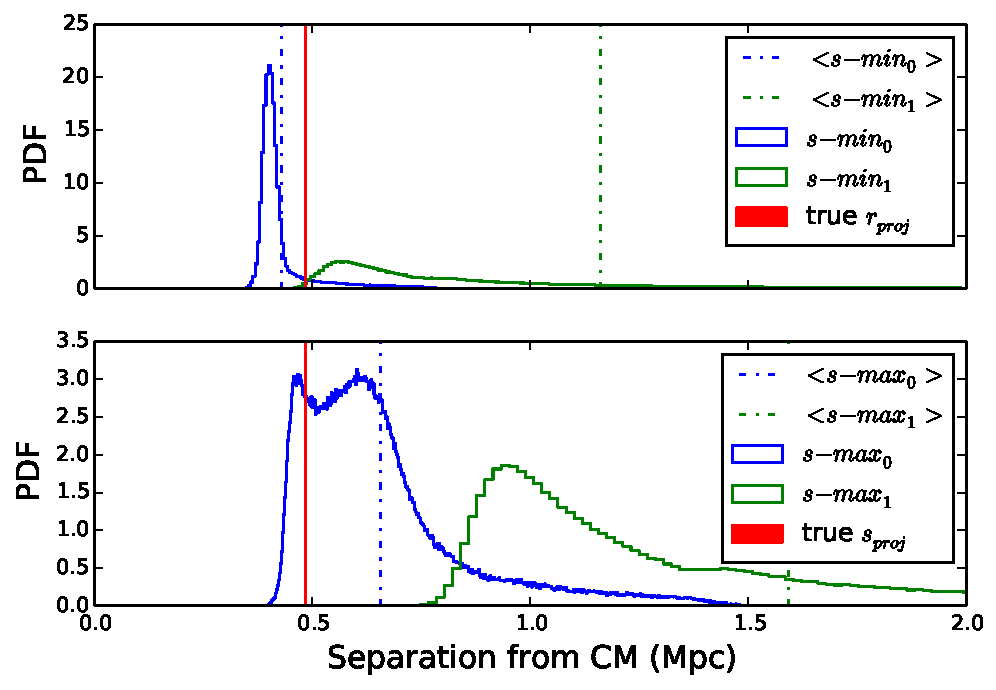
\includegraphics[width=\linewidth]{default_prior_bounds.pdf}
	\caption{Comparison of the observed position of the relic with the
	predicted position from the two simulated merger scenarios, with
	default prior applied to the PDFs.
	\label{fig: polarprior_bounds}}
\end{figure}




We present the PDFs of the inputs of the dynamical simulation and the
marginalized PDFs of the outputs after applying the polarization prior in
addition to the default priors. See following figure for explanations of
the order that we present the variables. 
\begin{figure}
	\begin{center}
	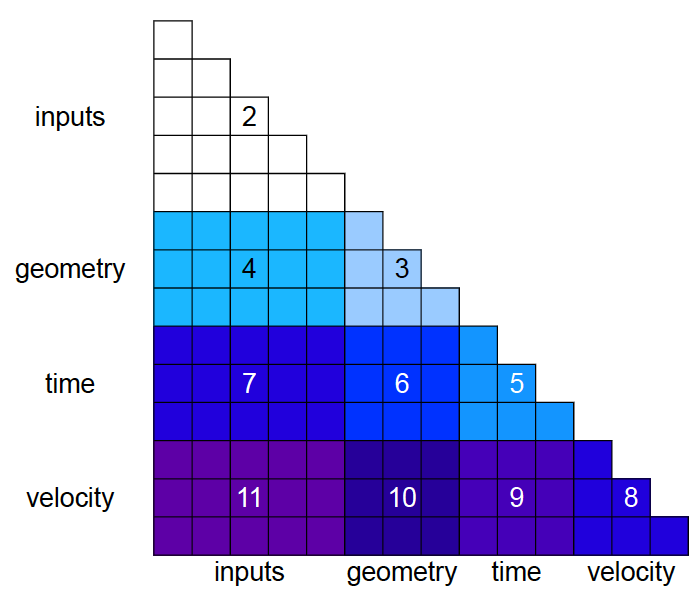
\includegraphics[width=\linewidth]{ElGordo_plot_config.png}
	\end{center}
	\caption{Matrix of variables used in the simulations. We present them in
	4 categories, including, inputs, geometry, time and velocity. Regions of
	the same color represent one plot and the number
indicates the corresponding figure number in this appendix.}
\end{figure}



%make use of subplots from matplotlib in order to plot all the posteriors
\label{app: results}

%%%%%%%%%%%%% TASK --- 

\clearpage
\begin{figure*}
	\begin{minipage}{180mm}
	\begin{center}
	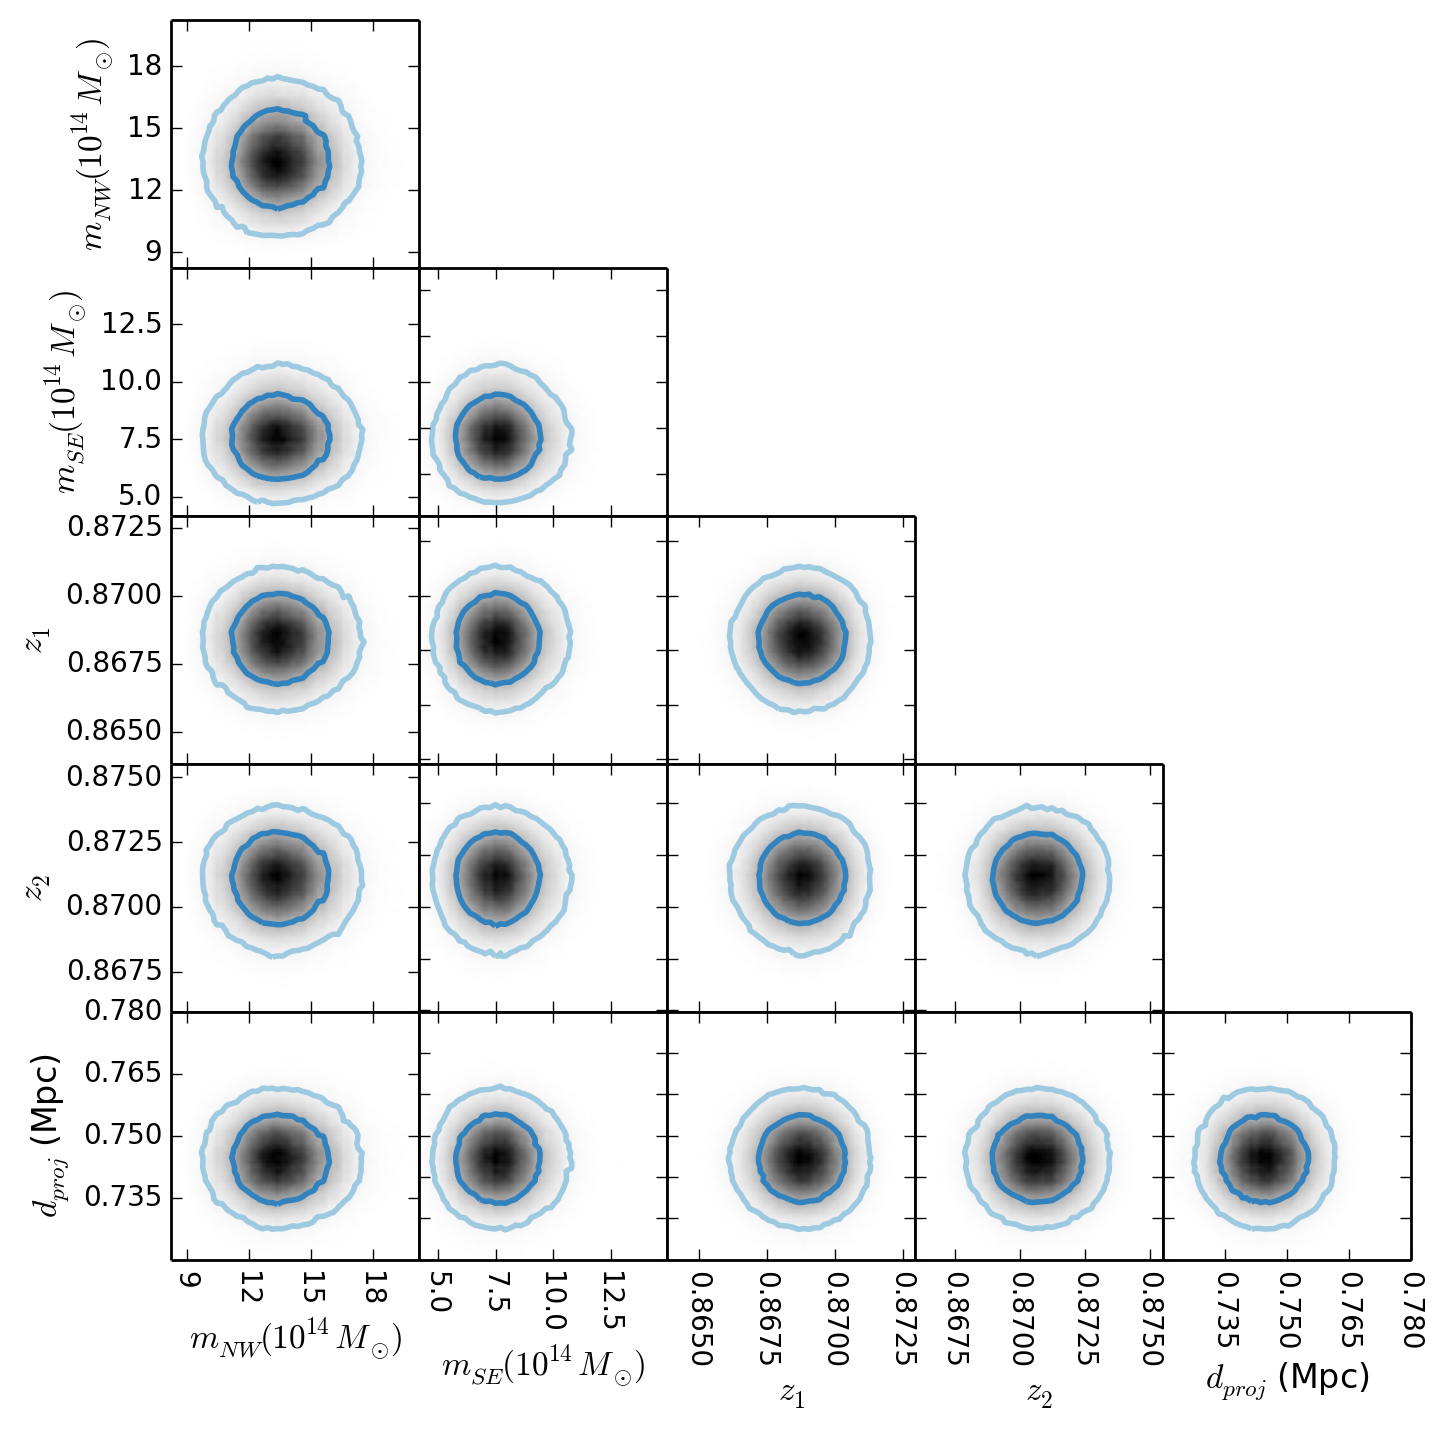
\includegraphics[width=0.65\linewidth]{TwoMnWBSG_inputsVsinput.png}
	\caption{Marginalized PDFs of original inputs (vertical axis) and the inputs after
applying polarization prior and default priors (horizontal axis). The inner and outer contour
denote the central 68\% and 95\% credible regions respectively.
The circular contours show that the application of priors did not introduce
uneven sampling of inputs. }
	\end{center}
	\end{minipage}
\end{figure*}

\begin{figure*}
\begin{minipage}{180mm}
	\begin{center}
	%\vspace{200px}
	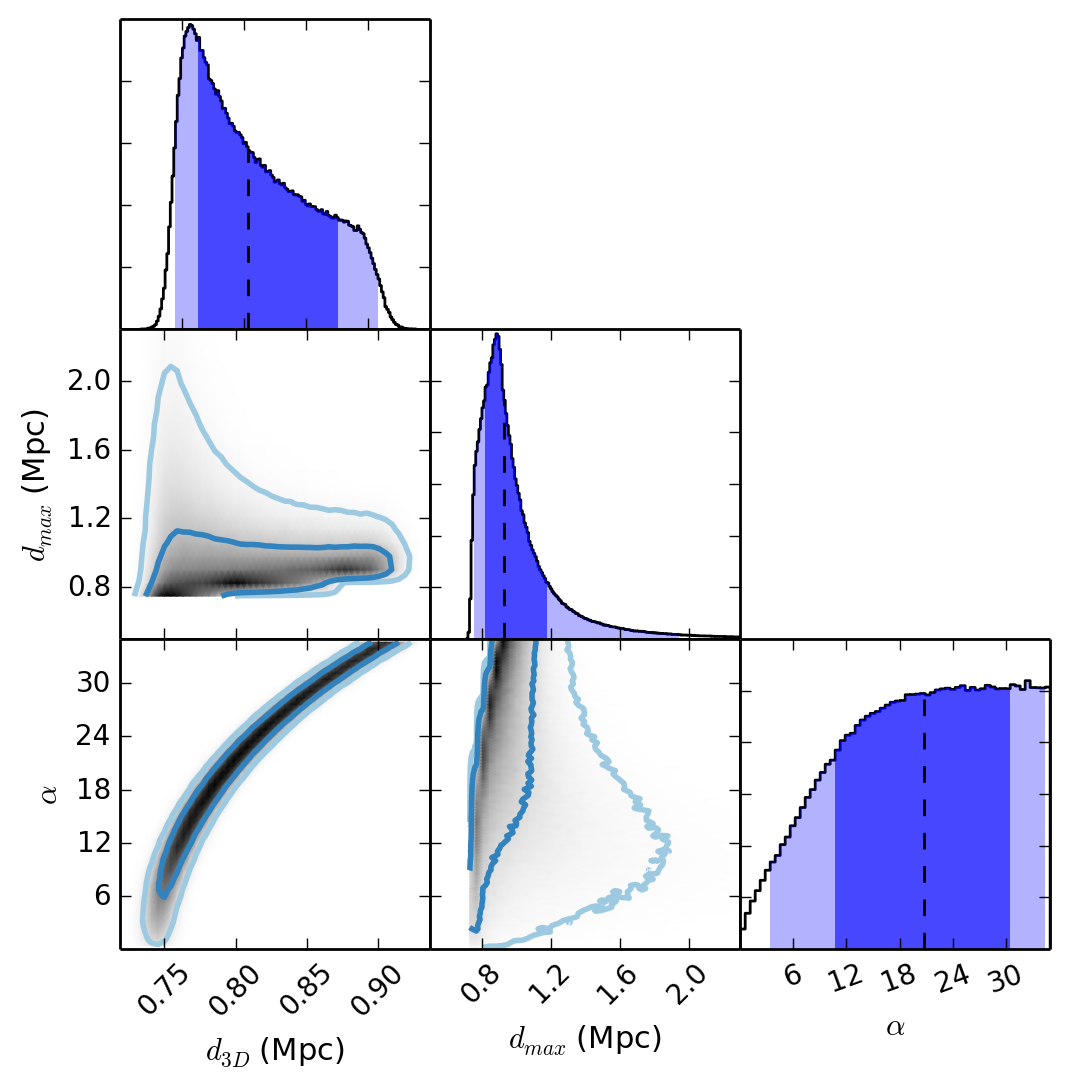
\includegraphics[width=0.5\linewidth]{TwoMnWBSG_tri_geo.png}
	\caption{One-dimensional marginalized PDFs (panels on the diagonal) and
		two-dimensional marginalized PDFs of variables
		denoting characteristic distances and projection angle of the mergers.}
	\end{center}
	\end{minipage}
\end{figure*}

\begin{figure*}
\begin{minipage}{180mm}
	\begin{center}
	%\vspace{200px}
	\includegraphics[width=0.7\linewidth]{TwoMnWBSG_geoVsinputs.png}
	\caption{Marginalized PDFs of characteristic distances and projection
		angle of the merger and the inputs of the simulation.}
	\end{center}
	\end{minipage}
\end{figure*}

\begin{figure*}
\begin{minipage}{180mm}
	\begin{center}
	%\vspace{200px}
	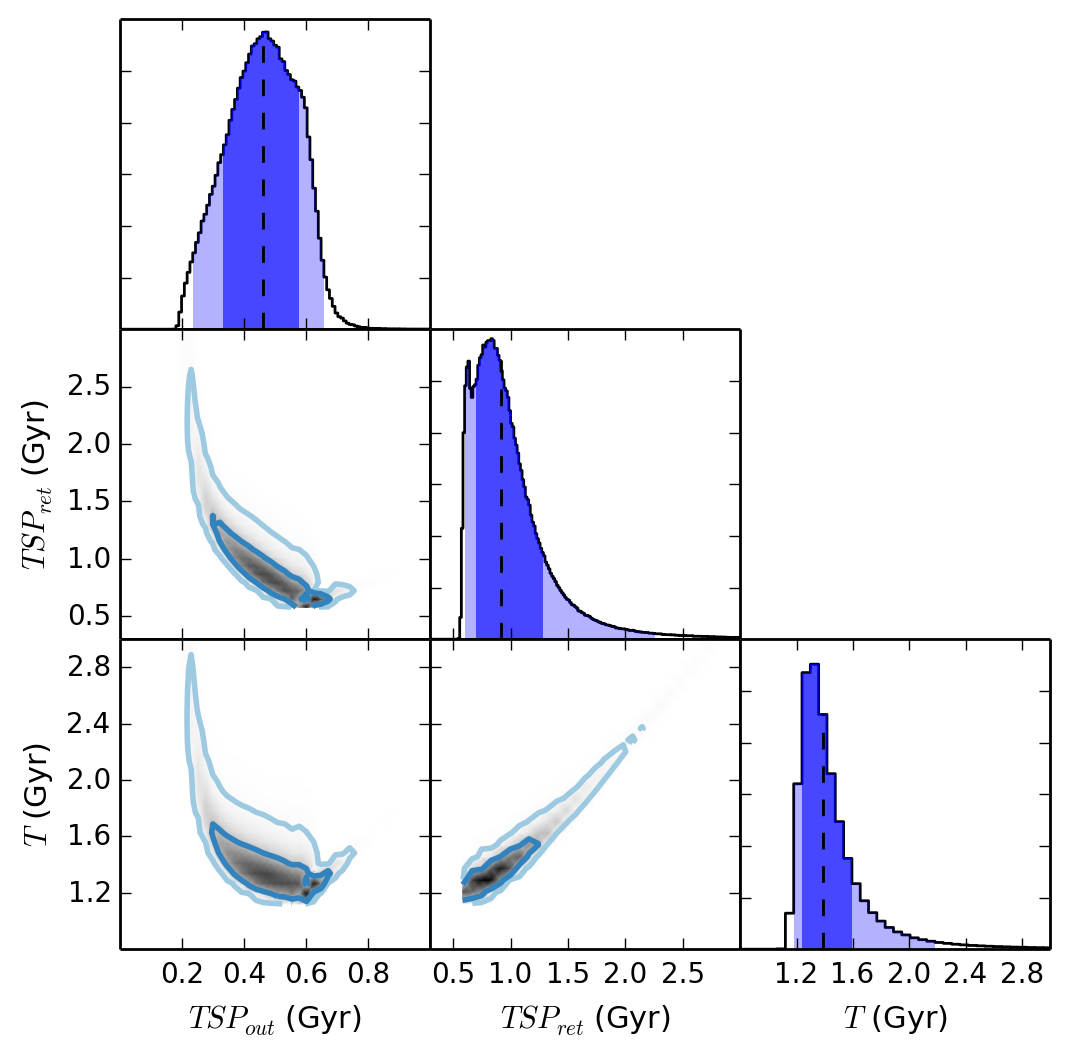
\includegraphics[width=0.5\linewidth]{TwoMnWBSG_tri_time.png}
	\caption{One-dimensional PDFs of characteristic timescales of the simulation
(panels on the diagonal) and the marginalized PDFs of different timescales.}
	\end{center}
\end{minipage}
\end{figure*}

\begin{figure*}
\begin{minipage}{180mm}
	\begin{center}
	%\vspace{200px}
	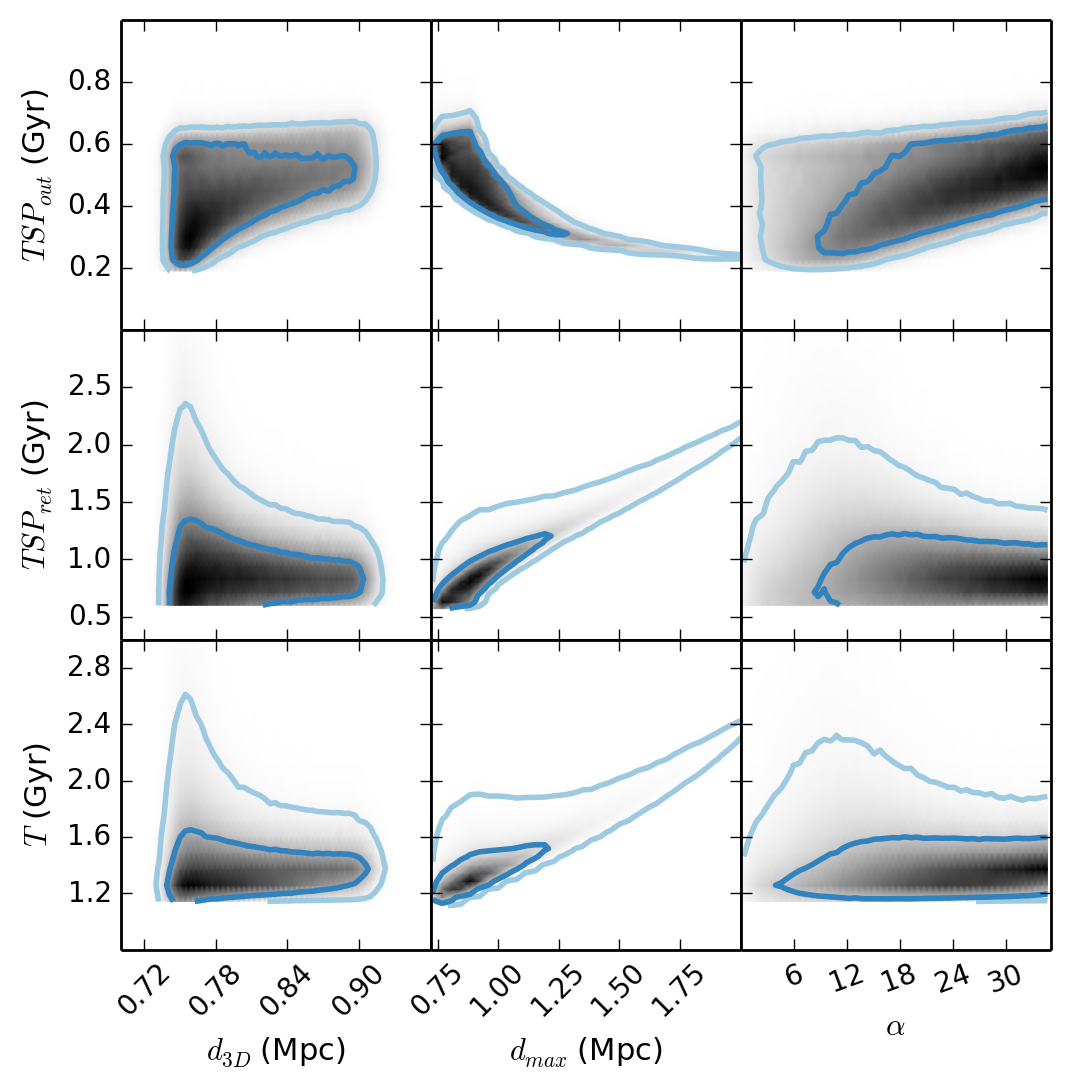
\includegraphics[width=0.5\linewidth]{TwoMnWBSG_timeVsgeo.png}
	\caption{Marginalized PDFs of characteristic timescales of the simulation
and the characteristic distances and the projection angle of the merger. }
	\end{center}
\end{minipage}

\end{figure*}

\begin{figure*}
\begin{minipage}{180mm}
	\begin{center}
	%\vspace{200px}
	\includegraphics[width=0.7\linewidth]{TwoMnWBSG_timeVsinput.png}
	\caption{Marginalized PDFs of characteristic timescales of the simulation
and the inputs.}
	\end{center}
\end{minipage}
\end{figure*}

\begin{figure*}
\begin{minipage}{180mm}
	\begin{center}
	%\vspace{200px}
	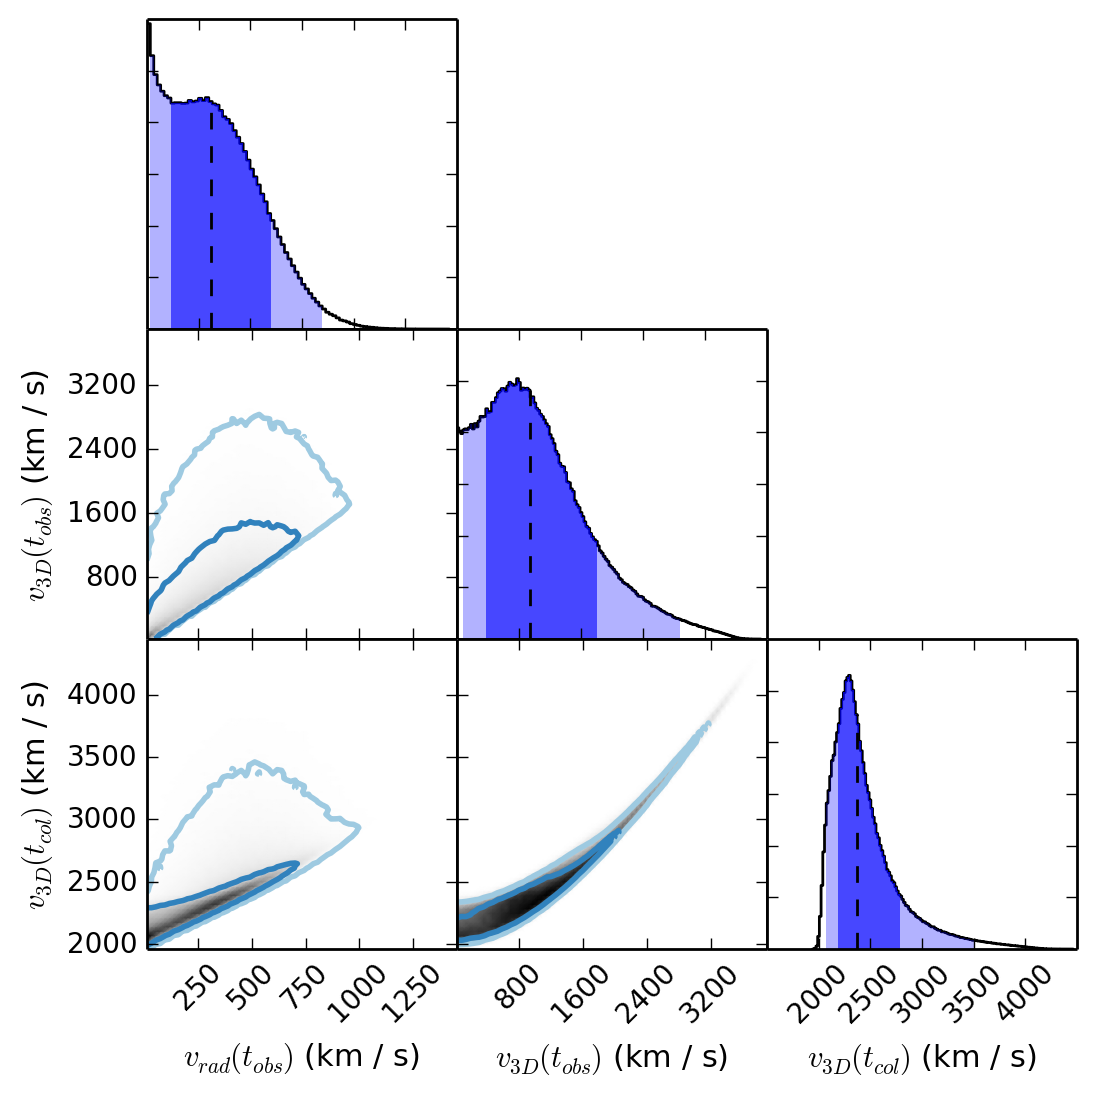
\includegraphics[width=0.5\linewidth]{TwoMnWBSG_tri_vel.png}
	\caption{One-dimensional marginalized PDFs of velocities at
	characteristic times (panels on the diagonal) and marginalized PDFs of
different velocities.}
	\end{center}
\end{minipage}
\end{figure*}

\begin{figure*}
\begin{minipage}{180mm}
	\begin{center}
	%\vspace{200px}
	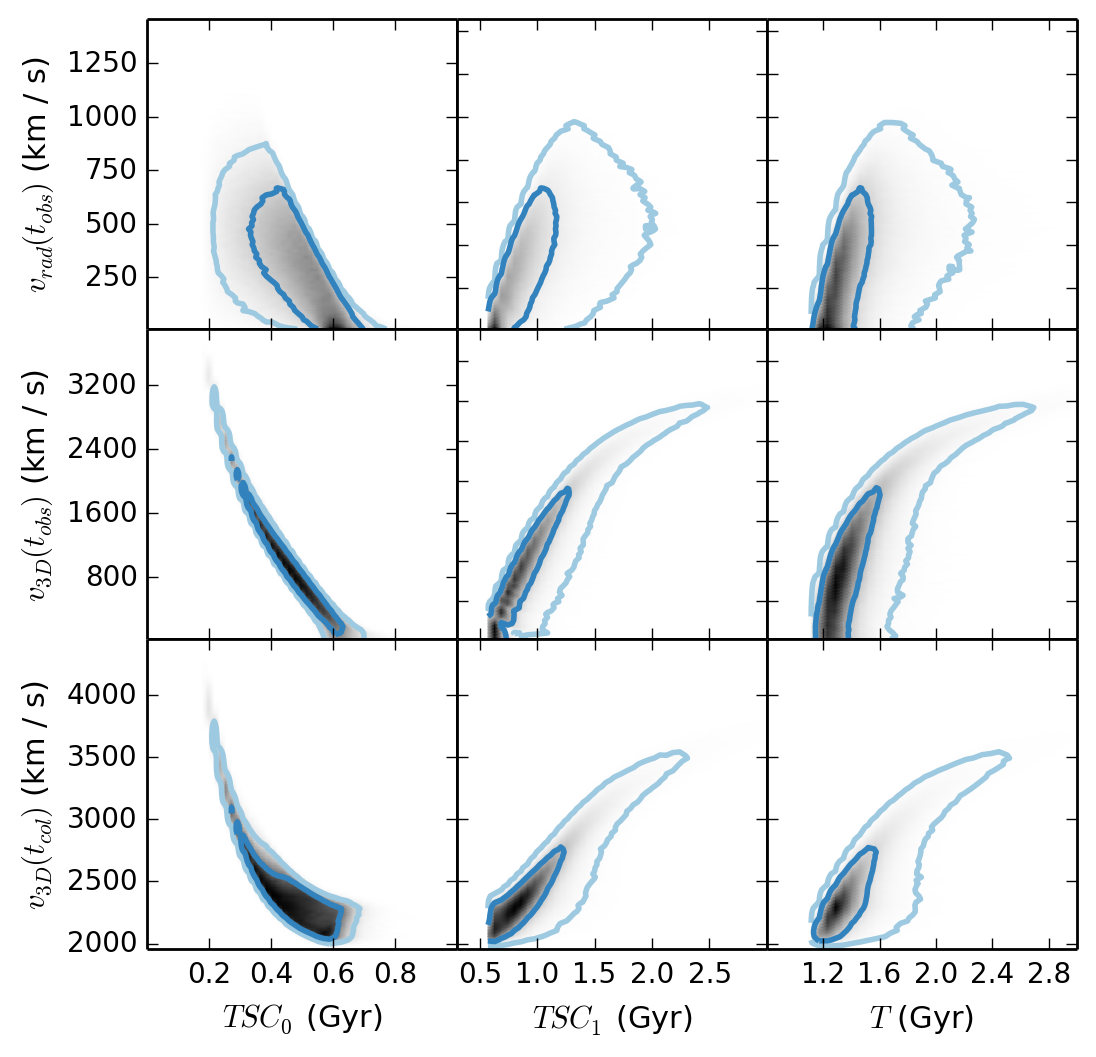
\includegraphics[width=0.5\linewidth]{TwoMnWBSG_velVStime.png}
	\caption{Marginalized PDFs velocities and the characteristic timescales
	of the simulation against the inputs.}
	\end{center}
\end{minipage}
\end{figure*}

\begin{figure*}
\begin{minipage}{180mm}
	\begin{center}
	%\vspace{200px}
	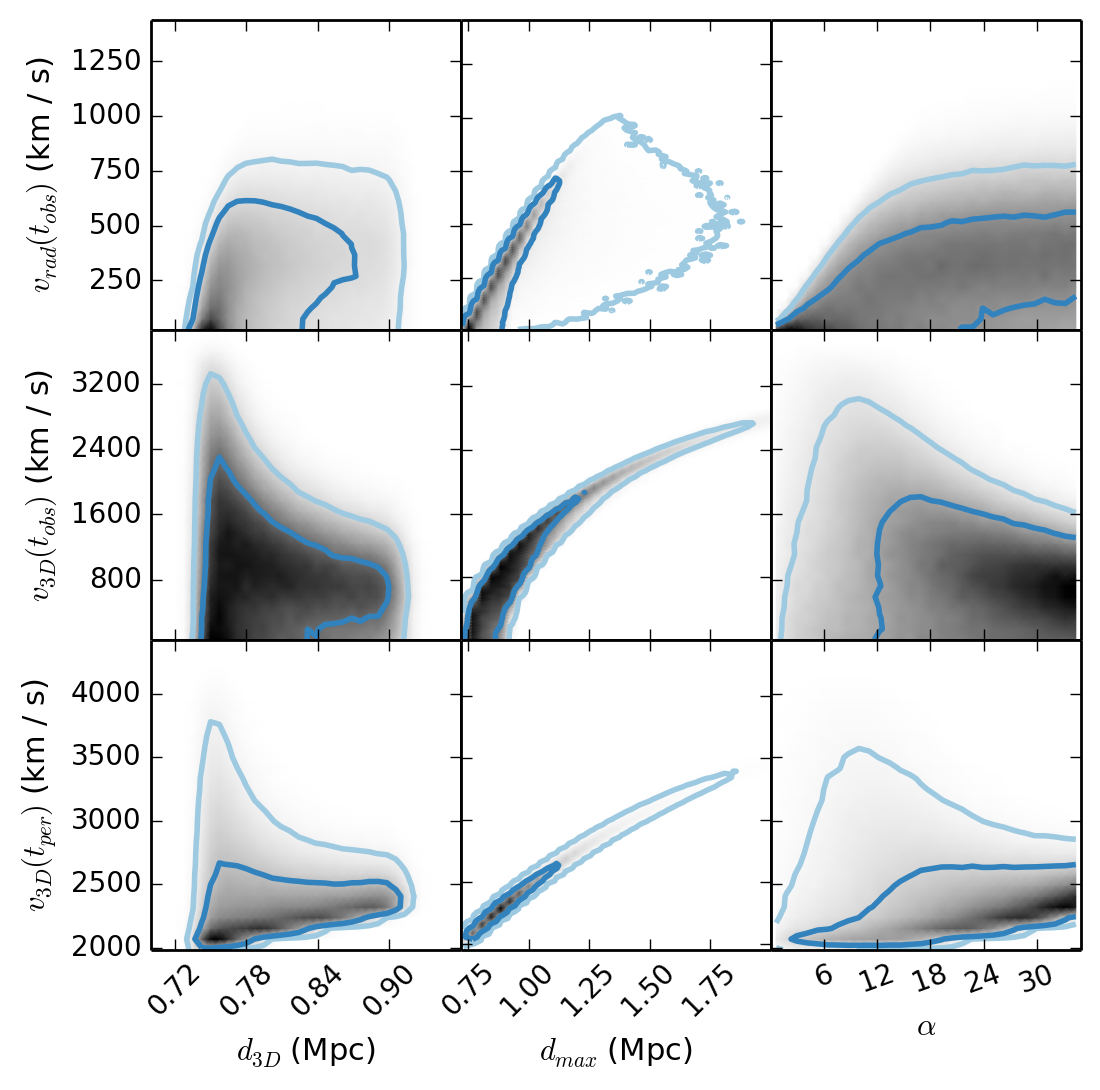
\includegraphics[width=0.5\linewidth]{TwoMnWBSG_velVSgeo.png}
	\caption{Marginalized PDFs of the velocities at characteristic timescales
		and the characteristic distances and the projection angle of the merger. }
	\end{center}
\end{minipage}
\end{figure*}

\begin{figure*}
\begin{minipage}{180mm}
	\begin{center}
	%\vspace{200px}
	\includegraphics[width=0.7\linewidth]{TwoMnWBSG_velVsinputs.png}
	\caption{Marginalized PDFs of relative velocities characteristic
	timescales of the simulation and the inputs.}
	\end{center}
\end{minipage}
\end{figure*}


\bsp 
\label{lastpage} 




\end{document}
